% 20241108
% Giovanni Ramirez
% ramirez@ecfm.usac.edu.gt

%
% Esta es una plantilla y contiene lo mínimo que debe llevar el
% informe final del año de prácticas.  La portada es una propuesta y
% se puede ajustar según se desee.
%
% Esta plantilla se puede usar tanto en un compilador de LaTeX en su
% computadora o en algún compilador en línea como overleaf.com
%

\documentclass[titlepage,11pt]{report}

%%% PAQUETES
% esto es para hacer las cosas en español y para usar el punto como separador
% decimal
\usepackage[spanish,es-nodecimaldot]{babel}%
% esto es por la codificación con la que se escribe, revisar la codificación
% de su sistema pues podría estar en utf16 o en iso-latin-1 o iso 8859-1
\usepackage[utf8]{inputenc}%
\usepackage{float}

\usepackage{listings}
\usepackage{xcolor} % para colores

\lstdefinelanguage{Mathematica}{
  morekeywords={
    Module, Table, Plot, Integrate, Sum, If, Do, While, For, Return,
    Function, Set, SetDelayed, Rule, RuleDelayed, Block, With, True, False
  },
  sensitive=true,
  morecomment=[l](\*),
  morestring=[b]",
}

\lstset{
  language=Mathematica,
  basicstyle=\ttfamily\small,
  keywordstyle=\color{blue}\bfseries,
  commentstyle=\color{gray},
  stringstyle=\color{red},
  showstringspaces=false,
  breaklines=true,
  postbreak=\mbox{\textcolor{gray}{$\hookrightarrow$}\space}
}
% esto es para agregar gráficas y figuras
\usepackage{graphicx}%
% esto es por algunos símbolos como la ñ o las vocales tildadas
\usepackage{latexsym}%
\usepackage{amsmath, amssymb, graphics, setspace}
\usepackage{xcolor} % Para colores
\usepackage{listings} % Para mostrar código
\usepackage[many]{tcolorbox} % Para cajas con estilo
\usepackage{geometry} % Para ajustar márgenes

% Configuración de listings para Mathematica

% esto es para tener acceso a varios símbolos matemáticos
\usepackage{amsfonts, amsmath}%
% esto es para facilitar la escritura de algunos símbolos en física
\usepackage{physics}
% esto es para poder usar el sistema internacional de unidades
\usepackage[amssymb]{SIunits}%
% esto es para que la página sea tamaño carta
\usepackage[letterpaper, bottom=25mm, top=25mm]{geometry}
% esto es para los colores, la opción table es para poner colores en las
% celdas

% esto es para las tablas largas
\usepackage{longtable}
% esto es para poder escribir en varios renglones en la tabla
\usepackage{array}

% esto es útil para los hipervínculos y metadata
\usepackage[bookmarksnumbered, breaklinks={true},%
pdfauthor={Bilbo Baggins (bilbo@theshire.middleearth)},%
pdftitle={El Hobbit o la historia de una ida y una vuelta},%
pdfsubject={Describir las aventuras de Bilbo},%
pdfkeywords={condensed matter materials \& applied physics, quasiparticles \&
  collective excitations, optical phonons}]{hyperref}


\begin{document}
% % % % % % % % % % % % % % % % % % % % % % % % % % % % % % % % % % %
% aquí se define la página de la portada, las distancias y tamaños son
% relativos al tamaño de la fuente que se define al inicio en documentclass
\begin{titlepage}
  % esto es para que no ponga número a la página
  \pagestyle{empty}
  % esto agrega el título a los bookmarks
  \pdfbookmark[0]{Title}{title}
  \begin{center}
    % esto es para los logos
    \begin{minipage}{\textwidth}
      \begin{minipage}[c]{0.45\textwidth}
        \centering \includegraphics[width=.8\textwidth]{usacAzul}
      \end{minipage}%
      \hfill
      \begin{minipage}[c]{0.45\textwidth}
        \vspace{-1em}\includegraphics[width=.85\textwidth]{ecfmAzul}
      \end{minipage}
    \end{minipage}

    % esto pone los nombres de las instituciones
    \vspace{2em}
    \begin{minipage}[t]{.95\textwidth}
      \centering\large
      \textsc{Universidad de San Carlos de Guatemala\\
        Escuela de Ciencias Físicas y Matemáticas}
    \end{minipage}

    % esto pone la línea horizontal
    \vspace{1em}\noindent\rule{\textwidth}{1px}\vfill
    % esto pone el título
    \begin{minipage}[t]{.95\textwidth}
      \centering\Huge
      \textsc{Reconstrucción no
paramétrica de funciones de
distribución de partones}
    \end{minipage}

    % esto pone los datos 
    \vfill
    \begin{minipage}[t]{.75\textwidth}
      \centering
      Informe final de prácticas elaborado por\\%
      \textbf{Miguel Alexander Avila Chacón}\\
      presentado ante el Departamento de Física
    \end{minipage}

    % esto pone más datos
    \vfill
    \begin{minipage}[t]{.95\textwidth}
      \centering
      Supervisado por \\%
      MSc. Elser Adolfo López Rosa
    \end{minipage}

    \vfill\noindent\rule{\textwidth}{1px}
    \begin{minipage}[t]{.95\textwidth}
      \centering
      Guatemala, agosto de 2025
    \end{minipage}
  \end{center}
\end{titlepage}
% % % % % % % % % % % % % % % % % % % % % % % % % % % % % % % % % % %


% esto hace que el resumen no tenga número de página y que la introducción
% empiece con el número de página 1
\pagestyle{empty}
\setcounter{page}{0}

% % % % % % % % % % % % % % % % % % % % % % % % % % % % % % % % % % %
% en esta página se hace un resumen del trabajo, se recomienda que no exceda
% las 500 palabras.
%

\section*{Resumen}
\label{sec:resumen}

% ver metadatos
\vspace{2em}
\textbf{Palabras clave:} parton distribution functions \& phenomenology \& high energy physics.

% esto es para terminar la página del resumen y pasar a la nueva página con el
% número uno
\newpage
\pagestyle{plain}

\chapter{Introducción}
\label{sec:introduccion}

Un partón es el nombre que recibe una partícula fundamental (como un quark o un gluón) dentro del interior de un hadrón, como el protón o el neutrón.

Las funciones de distribución de partones (PDFs por sus siglas en inglés) describen la probabilidad de encontrar un partón en el interior de un hadrón con un momento y energía determinados. Estas funciones son fundamentales para realizar predicciones en física de altas energías, como en los experimentos de colisionadores \cite{placakyte2011parton}. Este proyecto se enfoca en la reconstrucción de las PDFs mediante métodos no paramétricos.

Por lo general las PDFs se determinan a partir de parametrizaciones funcionales específicas que se ajustan a datos experimentales, como se observa en: \cite{Lopez2025}, \cite{Kovarik:2019xvh}, \cite{Dulat:2015mca}, \cite{Hou:2019efy}.

Este proyecto propone técnicas de reconstrucción no paramétricas, lo cual implica que no se asume una forma funcional específica para las PDFs, así, busca reconstruirlas directamente a partir de los datos. Se considerarán métodos de integración numérica en intervalos finitos. Este enfoque se encuentra en fase de desarrollo; se han explorado, por ejemplo, métodos bayesianos como en \cite{karpie2019reconstructing}, \cite{dutrieux2025simple}, \cite{candido2024bayesian}.

Uno de los fundamentos teóricos que motivan este trabajo es el problema truncado de momentos de Hausdorff, que consiste en determinar una distribución $\Phi(x)$ en el intervalo $[0,1]$ a partir de un número finito de sus momentos $\mu_n=\int d\Phi(x) x^{n-1}$, $n\in \mathbb{N}$, donde los $\mu_n$ forman una sucesión completamente monótona, lo que garantiza la unicidad de la solución \cite{Lopez2025}, \cite{garciaproblema}.

Este problema está totalmente determinado y tiene una solución única y completa cuando se conocen todos los momentos \cite{athanassoulis2002truncated}, \cite{gzyl2010hausdorff}, \cite{tagliani2011hausdorff}. En el contexto de la física de partículas, sólo suelen conocerse algunos momentos. Por lo que no es posible reconstruir de manera única la función original, esto convierte al problema en uno mal planteado desde el punto de vista matemático, requiriendo de herramientas extras para la construcción.

\chapter{Objetivos}
\label{sec:objetivos}
\section{General}
\label{sec:general}

Estudiar métodos no paramétricos para reconstruir funciones de distribución de partones a partir de sus momentos y datos simulados.

\section{Específicos}
\label{sec:especificos}

\begin{itemize}
    \item Estudiar las funciones de distribución de partones.

    \item Estudiar los distintos métodos de integración numérica.

    \item Analizar la eficacia de los distintos métodos para reconstruir las PDFs.
\end{itemize}


\chapter{Marco teórico}
\label{sec:marco}

\section{Función de distribución de partones}

Se le denomina partón a los constituyentes de un nucleón. Existen dos tipos conocidos de constituyentes de un nucleón: las partículas eléctricamente neutras llamadas gluones, y los fermiones de espín 1/2 denominados quarks, que definen el tipo de nucleón según su combinación \cite{Lopez2025}. \\



En la cromodinámica cuántica se conoce un tipo de interacción denominada \textit{dispersión inelástica profunda} (DIS por sus siglas en inglés) donde una partícula dispersa a otra, transfiriendo una gran cantidad de momento y energía. Se considera por ejemplo un proceso leptón-hadrón de la forma $l(k)+H(P)\to l(k')+X$, esto es, un leptón de cuadrimomento $k$ colisiona con un hadrón $H$ de masa $M$ y cuadrimomento $P$. El leptón tendrá en su estado final un cuadrimomento $k'$ y el fotón de interacción un cuadrimomento $q'=(k-k')$ \cite{doi:https://doi.org/10.1002/352760314X.ch2}. Desde el marco de referencia en reposo del objetivo, se pueden escribir las siguientes ecuaciones:
\begin{equation*}
    q^2=(k-k')^2=-Q^2<0,
\end{equation*}
\begin{equation*}
    \nu = P\cdot q=M(E-E').
\end{equation*}

El observable de interés en las interacciones DIS es la sección eficaz. Esta es proporcional al cuadrado de la amplitud de dispersión $|\mathcal{A}|^2$, que puede escribirse como la contracción de dos tensores, el leptónico $l^{\mu \nu}$ y el hadrónico $W^{\mu \nu}$ \cite{Lopez2025}. De la siguiente manera:
\begin{equation*}
    d\sigma \propto |\mathcal{A}|^1\propto l_{\mu\nu}W^{\mu\nu}.
\end{equation*}

El vértice leptónico puede describirse por medio de la electrodinámica cuántica de la siguiente forma:
\begin{equation*}
    l_{\mu\nu}=2\left(k'_\mu k_\nu+k'_\nu k_\mu+\frac{q^2}{2}g_{\mu\nu}\right).
\end{equation*}

Puede demostrarse que el tensor hadrónico puede parametrizarse de la siguiente forma:
\begin{align}\label{longW}\begin{split}
    W^{\mu\nu}=-\left(g^{\mu\nu}-\frac{q^{\mu}q^{\nu}}{q^2}\right)W_1(\nu, Q^2)+\left(P^{\mu}-q^{\mu}\frac{P\cdot q}{q^2}\right)\left(P^{\nu}-q^{\nu}\frac{P\cdot q}{q^2}\right)\frac{1}{M^2}W_2(\nu, Q^2)\\+\frac{i}{M^2}\epsilon_{\alpha}^{\mu\nu\alpha\beta}q_{\beta}W_3(\nu, Q^2), 
\end{split}
\end{align}

\noindent donde $\epsilon^{\mu\nu\alpha\beta}$ es el símbolo de Levi-Civita de 4 dimensiones y $W_1$, $W_2$ son las funciones electromagnéticas de estructura, y $W_3$ toma en cuenta las interacciones que envuelven corrientes de violación de paridad \cite{Lopez2025}. Al combinar estas dos ecuaciones se obtiene que la sección transversal no polarizada en el marco de referencia de laboratorio es:
\begin{equation*}
    \left.\frac{d^2\sigma}{dQ^2d\nu}\right|_{\text{Lab}}=\frac{\alpha}{4k^2\sin^{4}(\theta/2)}\frac{\pi}{kk'}[W_2(\nu, Q^2)\cos^2(\theta/2)+2W_1(\nu, Q^2)\sin^2(\theta/2)],
\end{equation*}

donde $Q^2=-q^2$ y $\nu$ es la energía transferida. \\

Bjorken propuso que para una interacción DIS con las siguientes condiciones:
\begin{equation}
    \left\{
\begin{array}{l}
Q^2 \to \infty \\
\nu \to \infty
\end{array}
\right. \quad \text{con } x = \frac{Q^2}{2(P \cdot q)}\ \text{finito}.
\end{equation}


Para $x$, una variable de escala que corresponde a la fracción total de momento de hadrón que acarrea cada constituyente individual, las funciones de estructura cumplirán:
\begin{equation*}
    MW_1(Q^2, \nu)\underset{Q^2 \to \infty}{\longrightarrow} F_1(x),
\end{equation*}
\begin{equation*}
    \nu W_2(Q^2, \nu)\underset{Q \to \infty}{\longrightarrow} F_2(x).
\end{equation*}

Esto es, las funciones se hacen finitas e independientes de $Q^2$ para un $x$ dado. \\

Ahora bien, se considera el límite de Bjorken para esta interacción, sea $m_i=\xi M$ la masa del i-ésimo constituyente y $e_i$ su carga. En este caso, $Q^2$ y $\nu$ son tales que los partones se consideran libres y acarrean una fracción de momento longitudinal $p_i^{\mu}=\xi P^{\mu}$. Sea $x$ tal que $x=z\xi$ donde $z=Q^2/(2p_i\cdot q)$ \cite{PhysRev.179.1547}. Entonces
\begin{equation*}
    \left.\frac{d^2\sigma}{dQ^2d\nu}\right|_{\text{Lab}}=\frac{\alpha}{4k^2\sin^{4}(\theta/2)}\frac{\pi}{kk'}[e_i^2\cos^2(\theta/2)+2e_i\frac{Q^2}{4m_i^2}\sin^2(\theta/2)]\delta\left(\nu-\frac{Q^2}{2m_i}\right),
\end{equation*}

\noindent y por tanto puede escribirse que:
\begin{equation}\label{Wbar1}
    \tilde{W}_1^i=e_i^2\frac{Q^2}{4m_i^2}\delta\left(\nu-\frac{Q^2}{2m_i}\right)=\frac{e_ix^2}{2\xi M}\delta(\xi-x),
\end{equation}
\begin{equation}\label{Wbar2}
    \tilde{W}_2^i=e_i^2\delta\left(\nu-\frac{Q^2}{2m_i}\right)=\frac{2e_i^2M\xi x^2}{Q^2}\delta(\xi-x).
\end{equation}

El tensor hadrónico puede interpretarse también como la suma probabilística de todos sus tipos de partones constituyentes. Así, un tensor partónico $\tilde{W}_i^{\mu\nu}(z,Q^2)$, donde $Q^2$ es la magnitud del cuadrimomento \cite{10.1063/PT.3.2624}. Puede escribirse que:
\begin{align}\label{newW}
    W^{\mu\nu}=\int_0^{1}dz\int_0^{1}d\xi \sum_if^{i}(\xi, Q^2)\tilde{W}_i^{\mu\nu}(z,Q^2)\delta(x-z\xi)=\int_x^{1}\frac{d\xi}{\xi}\sum_{i}f^i(\xi, Q^2)\tilde{W_i}^{\mu\nu}\left(\frac{x}{\xi}, Q^2\right),
\end{align}

\noindent se puede escribir además que:
\begin{equation}\label{barW}
    \tilde{W}^{\mu\nu}=-\left(g^{\mu\nu}-\frac{q^{\mu}q^{\nu}}{q^2}\right)\tilde{W}_1^i(\nu, Q^2)+\left(p^{\mu}-q^{\mu}\frac{p\cdot q}{q^2}\right)\left(p^{\nu}-q^{\nu}\frac{p\cdot q}{q^2}\right)\frac{1}{\xi^2 M^2}\tilde{W}_2^i(\xi, Q^2),
\end{equation}

al combinar \ref{barW} con \ref{newW} y comparando con \ref{longW}, se llega al siguiente resultado para las funciones de estructura electromagnética:
\begin{equation*}
    W_k(x,Q^2)=\int_0^{1}\frac{d\xi}{\xi}\sum_if_i(\xi)\tilde{W}_k^i(\xi, Q^2),
\end{equation*}

\noindent para $k=1,2$. Así, con base en las ecuaciones \ref{Wbar1} y \ref{Wbar2}, se tiene que:
\begin{equation*}
    W_1(x,Q^2)=\frac{e_i^2}{2M}\sum_ie_i^2f_i(x),
\end{equation*}
\begin{equation*}
    W_2(x,Q^2)=\frac{x}{\nu}\sum_ie_i^2f_i(x),
\end{equation*}

Finalmente, es posible definir las funciones $F_k(x)$, $k=1,2$ tales que:
\begin{equation}
    F_1(x)\equiv MW_1=\frac{1}{2}\sum_ie_i^2f_i(x),
\end{equation}
\begin{equation}
    F_2(x)\equiv \nu W_2=x\sum_ie_i^2f_i(x),
\end{equation}

\noindent que son independientes de $Q^2$ tal como predice el límite de Bjorken. A la función $f_i(x)$ se le denomina \textbf{función de distribución de partones} y mide la distribución del momento de los quarks en el hadrón \cite{Lopez2025}. 

\section{Momentos de Mellin de la PDF}


Se define al n-ésimo momento de Mellin de la función de distribución de partones como:
\begin{equation*}
    \langle x^n\rangle_q=\int_0^{1}dx\ x^{n-1}f^{q}(x,Q^2),\ n=1,2,3, ...,
\end{equation*}

\noindent donde $q$ es el índice de sabor del quark. La distribución de quarks dentro de un hadrón debe satisfacer restricciones relacionadas a la cantidad de quarks y el momento \cite{Lopez2025}. Por ejemplo, la regla de suma de momentos satisface que:
\begin{equation*}
    \sum_{q}\langle x^2\rangle_q=\sum_{q}\int_0^{1}dx\ xf_1^{q}(x,Q^2)=1,
\end{equation*}

\noindent y se tiene que el contenido de quarks dentro de un hadrón está dado por:
\begin{equation*}
    \langle x^1\rangle_{q-\bar{q}}=\sum_{q}\int_0^{1}dx\ [f_1^{q}(x,Q^2)-f_1^{\bar{q}}(x,Q^2)]=N_{q},
\end{equation*}

\noindent dado un conjunto de momentos de Mellin es posible reproducir la función de distribución de partones. Para $f$ definida en $0<x<1$, se denomina a este problema como el \textit{problema de momentos de Hausdorff}.


\section{Problema de momentos de Hausdorff}

En general, dada una función $\Phi(x)$ definida en un intervalo $I$ con momentos $\mu_m$ tales que:
\begin{equation*}
    \mu_m=\int_Id\Phi x^{m-1},\ m=1,2,3, ...
\end{equation*}

El problema de momentos consiste en encontrar las condiciones que permiten que $\Phi(x)$ pueda ser reconstruida a partir de sus momentos \cite{alma99671493502466}. Si la solución es única, se considera un \textit{problema de momentos determinado}. En particular, se denomina al problema de momentos determinado en el intervalo $I=[0,1]$, como el problema de momentos de Hausdorff \cite{Hausdorff1923}. \\

Ahora bien, para que función no negativa $\Phi(x)$ tenga una solución única, la condición necesaria y suficiente es que su secuencia de momentos $\{\mu_{m}\}$ forme una secuencia completamente monótona. Además, una secuencia completamente monótona $\{\mu_m\}$ sujeta a la condición de normalización $\mu_1=1$ coincide con la secuencia de momentos de una única distribución de probabilidad. Este es el caso de la función de distribución de partones \cite{gzyl2010hausdorff}. \\

Generalmente se utilizan métodos paramétricos para reconstruir estas funciones. En este documento se mostrará el uso de una metodología no paramétrica a partir de tres distintos métodos de integración numérica: método del trapecio, método de Simpson y método de Gauss.

\section{Métodos de integración numérica}

\subsection{Método del trapecio}

La regla del trapecio aproxima la integral de una función $f(x)$ en el intervalo $I=[a,b]$ de la siguiente forma \cite{davis2007methods}:
\begin{equation*}
    \int_{a}^{b}f(x)dx\approx \frac{f(a)+f(b)}{2}(b-a)
\end{equation*}

Con un error global correspondiente a:
\begin{equation*}
    E=-\frac{1}{12}f''(\omega)(b-a)^3
\end{equation*}

Con $\omega\in I$ \cite{larson2005cálculo}.

\subsection{Método de Simpson}

La regla de Simpson establece la siguiente aproximación para la integral de $f(x)$ en $I=[a,b]$ \cite{davis2007methods}:
\begin{equation*}
    \int_{a}^{b}f(x)dx\approx \frac{(b-a)}{6}\left[f(a)+4f\left(\frac{a+b}{2}\right)+f(b)\right]
\end{equation*}

Con un error de cuadratura asociado de:
\begin{equation*}
    E(\xi)=-\frac{h^5}{90}f^{(4)}(\xi)
\end{equation*}

Donde $h=(b-a)/2$ y $\xi\in I$ \cite{07a21022-7e5e-3495-8122-12bedc23c3f3}.

\subsection{Método de Gauss}

La cuadratura de Gauss establece la siguiente aproximación para la integral de $f(x)$ en $I=[-1,1]$ \cite{burden2015numerical}:
\begin{equation*}
    \int_{-1}^{1}f(x)dx\approx \sum_{n=1}^{\infty}w_if(x_i)
\end{equation*}

También se conoce como método de Gauss-Legendre porque los coeficientes se relacionan con los polinomios de Legendre $P_n(x)$ de la siguiente manera:
\begin{equation*}
    w_i=\frac{2}{(1-x_i)[P'_n(x_i)]^2}
\end{equation*}

Donde $x_i$ son las raíces de dicho polinomio.

El error de cuadratura, es en este caso proporcional a la derivada $2n$-ésima. Esto es:
\begin{equation*}
    E(\xi)=\frac{(n!)^4}{(2n+1)[(2n)!)^3]}f^{(2n)}(\xi)
\end{equation*}

Para $\xi\in I$.


\chapter{Metodología}
\label{sec:metodologia}

El código de Mathematica utilizado para aproximar las PDFs tiene la siguiente teoría como base:

\section{Análisis}

Se parte de una función original $\phi(x)$ normalizada en $[0,1]$.

Los momentos están dados por:
\begin{equation*}
    \mu_n = \int_0^1 \phi(x) x^{n-1} \, dx, \quad n = 1, \dots, N.
\end{equation*}
    
Ahora se tiene la aproximación de $\phi(x)$.
\begin{equation*}
    \phi(x)\approx f(x)=\sum_{i=0}^{N-1} c_i x^i,
\end{equation*}

\noindent donde el objetivo es encontrar los coeficientes $c_i$. Los momentos $\mu_n$ pueden aproximarse mediante cuadratura de Gauss-Legendre. Dado que esta cuadratura está definida en $[-1,1]$, se hace un cambio de variable para integrarla en $[0,1]$, usando
\begin{equation*}
    \int_{a}^{b}\phi(x)dx=\frac{b-a}{2}\int_{-1}^{1}\phi\left(\frac{b-a}{2}u+\frac{b+a}{2}\right)du\approx \frac{b-a}{2}\sum_{j=1}^{M}\omega_j\phi\left(\frac{b-a}{2}u_j+\frac{b+a}{2}\right),
\end{equation*}

\noindent donde $\{u_j\}$ y $\{\omega_j\}$ son los puntos de evaluación y pesos en $[-1,1]$. Entonces para el intervalo $[0,1]$ se cumple que:
\begin{equation*}
    x_j = \frac{1}{2}(u_j + 1), \quad w_j = \frac{1}{2} \omega_j,
\end{equation*}

\noindent entonces, el momento se aproxima por:
\begin{equation*}
    \mu_n \approx \sum_{j=1}^{M} w_j \, \phi(x_j) \, x_j^{n-1}.
\end{equation*}


Los coeficientes $c_i$ son tales que los momentos de $f(x)$ coincidan con los de $\phi(x)$.
\begin{equation*}
    (\mu_n)_{f(x)} = \int_0^1 f(x) x^{n-1} dx = \int_0^1 \left( \sum_{i=0}^{N-1} c_i x^i \right) x^{n-1} dx = \sum_{i=0}^{N-1} c_i \int_0^1 x^{i+n-1} dx,
\end{equation*}

\noindent luego se pueden definir las entradas de una matriz $A$ tal que:
\begin{equation}\label{matrix}
    A_{ni} = \int_0^1 x^i x^{n-1} dx \approx \sum_{j=1}^{M} w_j x_j^{i + n -1}.
\end{equation}

\noindent así, se obtienen los coeficientes del polinomio mediante la ecuación:
\begin{equation}\label{sis}
    \vec{c} = A^T(AA^T)^{-1}\vec{\mu},
\end{equation}

\noindent aplicable tanto para sistemas determinados como indeterminados. Para el caso de la regla de Simpson se parte de una función original $\phi(x)$ normalizada en $[0,1]$. En particular, este método requiere de un número par $M$ de subintervalos con pasos equiespaciados $h=1/M$ y nodos $x_i=ih$, tal que $i=0,1,\cdots M$. Y el único cambio en el análisis se da en la definición de pesos es el siguiente:
\begin{equation*}
    w_j = \left\{ \begin{array}{lcc} h/3, \ j=0, j=M \\ 
    4h/3, \ j\ \text{mod}\ 2=1\\
    2h/3, \ j\ \text{mod}\ 2=0,\end{array}\right.
\end{equation*}

\noindent nuevamente se cumple la ecuación \ref{sis} para $A$ tal que cumple la ecuación \ref{matrix}. \\

Para el caso de la regla del trapecio se consideran $M$ subntervalos de nodos equiespaciados con paso $h=1/M$ tal que sus nodos son $x_i=ih$, $i=0, 1, 2,\cdots, M$. Los pesos son:
\begin{equation*}
    w_j = \left\{ \begin{array}{lcc} h/2,\ \ \ \ j=0, j=M \\
    h, \ \ \ \ \text{cualquier otro caso,} \end{array}\right.
\end{equation*}


\noindent teniendo finalmente la matriz $A$ definida según \ref{matrix} tal que $\vec{c} = A^T(AA^T)^{-1}\vec{\mu}$.

\section{Programación}

El código se divide en dos partes principales, la primera corresponde al cálculo de la función aproximada y el error global asociado a cada método, así como el error por punto, diferencia entre lo que se considera la función original, análoga a una función obtenida de forma experimental y la función aproximada.

Para simular la función original de distribución de partones se consideró la distribución beta. Para la cual se tiene una densidad de probabilidad definida en el intervalo $[0,1]$ tal que:
\begin{equation*}
    \phi(x)=\frac{x^{\alpha-1}(1-x)^{\beta-1}}{B(\alpha, \beta)}
\end{equation*}

Donde $B(\alpha,\beta)$ es la función beta y se define para $\alpha,\beta>0$ como:
\begin{equation*}
    B(\alpha,\beta)=\int_0^{1}x^{\alpha-1}(1-x)^{\beta-1}dx,
\end{equation*}

y es tal que:
\begin{equation*}
    B(\alpha,\beta)=B(\beta, \alpha)
\end{equation*}
\begin{equation*}
    B(\alpha,\beta)=\frac{\Gamma(\alpha)\Gamma(\beta)}{\Gamma(\alpha+\beta)}
\end{equation*}

Así, se consideró el siguiente código en Mathematica:
\begin{lstlisting}
Needs["NumericalDifferentialEquationAnalysis`"];

reconstruirBetaConError[metodo_, Nmomentos_, alpha_, beta_, 
  nPuntos_] := 
 Module[{psi, phiOriginal, x, w, potenciaSegura, mu, A, c, 
   phiRecSinTruncar, phiRec, nIntervals, puntosPesos, xQuad, wQuad, h,
    derivada2, derivada4, errorEst, puntosPesosMenos, xMenos, wMenos, 
   muMenos, cMenos, phiRecMenosSinTruncar, phiRecMenos, fineX, 
   originalFine, recFine, errorFine, maxError, rmse, selectedX, 
   tableData, plotError, plots, errorData, puntosMuestra, diff}, 
  psi[i_, x_] := If[i == 0, 1, x^i];
  phiOriginal[x_] := PDF[BetaDistribution[alpha, beta], x];
  potenciaSegura[lista_, k_] := 
   Table[If[k == 0, 1, If[lista[[i]] == 0, 0, lista[[i]]^k]], {i, 
     Length[lista]}];
  Which[metodo == "Trapecio", h = 1.0/nPuntos;
   x = Range[0, 1, h];
   w = ConstantArray[h, Length[x]];
   w[[1]] = h/2; w[[-1]] = h/2, metodo == "Simpson", 
   nIntervals = If[EvenQ[nPuntos], nPuntos, nPuntos + 1];
   h = 1.0/nIntervals;
   x = Table[i*h, {i, 0, nIntervals}];
   w = Table[
     Which[i == 0 || i == nIntervals, h/3, OddQ[i], 4*h/3, EvenQ[i], 
      2*h/3], {i, 0, nIntervals}], metodo == "Gauss", 
   puntosPesos = GaussianQuadratureWeights[nPuntos, 0, 1];
   {x, w} = Transpose[puntosPesos]];
  mu = Table[
    w . (phiOriginal[x]*potenciaSegura[x, n - 1]), {n, 1, 
     Nmomentos}];
  A = Table[
    w . potenciaSegura[x, j + n - 1], {n, 1, Nmomentos}, {j, 0, 
     Nmomentos - 1}];
  c = LeastSquares[A, mu];
  phiRecSinTruncar[x_] := 
   Sum[c[[i + 1]]*psi[i, x], {i, 0, Nmomentos - 1}];
  phiRec[x_] := Max[0, phiRecSinTruncar[x]];
  errorEst = 
   Which[metodo == "Trapecio", 
    derivada2 = {(-3 phiRecSinTruncar[0] + 4 phiRecSinTruncar[h] - 
         phiRecSinTruncar[2 h])/(2 h), (3 phiRecSinTruncar[1] - 
         4 phiRecSinTruncar[1 - h] + phiRecSinTruncar[1 - 2 h])/(2 h)};
    Abs[h^2/12 (derivada2[[2]] - derivada2[[1]])], 
    metodo == "Simpson", 
    derivada4 = {(-14 phiRecSinTruncar[0] + 72 phiRecSinTruncar[h] - 
         156 phiRecSinTruncar[2 h] + 168 phiRecSinTruncar[3 h] - 
         70 phiRecSinTruncar[4 h])/(24 h^3), (14 phiRecSinTruncar[
           1] - 72 phiRecSinTruncar[1 - h] + 
         156 phiRecSinTruncar[1 - 2 h] - 
         168 phiRecSinTruncar[1 - 3 h] + 
         70 phiRecSinTruncar[1 - 4 h])/(24 h^3)};
    Abs[h^4/180 (derivada4[[2]] - derivada4[[1]])], metodo == "Gauss",
     If[nPuntos > 1, 
     puntosPesosMenos = GaussianQuadratureWeights[nPuntos - 1, 0, 1];
     {xMenos, wMenos} = Transpose[puntosPesosMenos];
     muMenos = 
      Table[wMenos . (phiOriginal[xMenos]*
          potenciaSegura[xMenos, n - 1]), {n, 1, Nmomentos}];
     A = 
      Table[wMenos . potenciaSegura[xMenos, j + n - 1], {n, 1, 
        Nmomentos}, {j, 0, Nmomentos - 1}];
     cMenos = LeastSquares[A, muMenos];
     phiRecMenosSinTruncar[x_] := 
      Sum[cMenos[[i + 1]]*psi[i, x], {i, 0, Nmomentos - 1}];
     phiRecMenos[x_] := Max[0, phiRecMenosSinTruncar[x]];
     puntosMuestra = Range[0, 1, 0.01];
     diff = 
      Abs[phiRecSinTruncar[#] - phiRecMenosSinTruncar[#]] & /@ 
       puntosMuestra;
     Max[diff], 0], _, 0];
  fineX = Range[0, 1, 0.01];
  originalFine = phiOriginal /@ fineX;
  recFine = phiRec /@ fineX;
  errorFine = Abs[recFine - originalFine];
  maxError = Max[errorFine];
  rmse = Sqrt[Mean[errorFine^2]];
  selectedX = Range[0, 1, 0.1];
  tableData = 
   Table[{x, phiOriginal[x], phiRec[x], 
     Abs[phiOriginal[x] - phiRec[x]]}, {x, selectedX}];
  plots = {Plot[{phiOriginal[x], phiRec[x]}, {x, 0, 1}, 
     PlotStyle -> {Directive[Gray, Dashed], Directive[Blue, Thick]}, 
     PlotLegends -> {"Original", "Reconstruida (" <> metodo <> ")"}, 
     AxesLabel -> {"x", "\[Phi](x)"}, GridLines -> Automatic, 
     PlotLabel -> 
      "Reconstrucción con " <> metodo <> 
       "\nError cuadratura estimado: " <> 
       ToString[NumberForm[errorEst, 4]], ImageSize -> 300], 
    ListLinePlot[Transpose[{fineX, errorFine}], 
     PlotLabel -> 
      "Error puntual: max = " <> ToString[NumberForm[maxError, 4]] <> 
       ", RMSE = " <> ToString[NumberForm[rmse, 4]], 
     AxesLabel -> {"x", "Error"}, GridLines -> Automatic, 
     ImageSize -> 300]};
  Print[Grid[{plots}, Spacings -> {2, 0}]];
  Print["\nTabla comparativa en puntos seleccionados:"];
  Print[Grid[
    Prepend[tableData, {"x", "Original", "Reconstruida", 
      "Error |Original - Reconstruida|"}], Frame -> All, 
    Alignment -> {Center, Center}, 
    Background -> {None, {LightBlue, None}}]];
  <|"PhiOriginal" -> phiOriginal, "PhiRec" -> phiRec, 
   "Puntos" -> fineX, "Errores" -> errorFine, "MaxError" -> maxError, 
   "RMSE" -> rmse|>]
\end{lstlisting}


Se consideró además una segunda función, tal que analiza cómo mejora la precisión entre la función original y la aproximada a medida que crece el número de momentos conocidos para un número de puntos dado:
\begin{lstlisting}
analizarPrecisionPorMomentos[metodo_, alpha_, beta_, nPuntos_, 
  momentoInicial_, momentoFinal_] := 
 Module[{rangomomentos, resultados, erroresMaximos, rmses}, 
  rangomomentos = Range[momentoInicial, momentoFinal];
  resultados = 
   Table[reconstruirBetaConError[metodo, n, alpha, beta, nPuntos], {n,
      rangomomentos}];
  erroresMaximos = resultados[[All, "MaxError"]];
  rmses = resultados[[All, "RMSE"]];
  Print[ListLogPlot[{Transpose[{rangomomentos, erroresMaximos}], 
     Transpose[{rangomomentos, rmses}]}, 
    PlotLegends -> {"Error Máximo", "RMSE"}, 
    PlotLabel -> "Mejora de Precisión con el Aumento de Momentos", 
    AxesLabel -> {"Número de Momentos", "Error"}, 
    GridLines -> Automatic, ImageSize -> 600]];
  Print["\nTabla de mejora de precisión:"];
  Grid[Prepend[
    Transpose[{rangomomentos, erroresMaximos, rmses}], {"# Momentos", 
     "Error Máximo", "RMSE"}], Frame -> All, 
   Alignment -> {Center, Center}, 
   Background -> {None, {LightBlue, None}}]]
\end{lstlisting}

Se impuso además la condición para la función reconstruida de ser siempre positiva, para representar con propiedad una distribución de probabilidad como es la función de distribución de partones.

Puesto que el coste computacional de calcular una derivada $2n$-ésima como es el caso del error en cuadratura correspondiente al método de Gauss, se estimó una cota superior de este error mediante la comparación de la reconstrucción con $n$ y $n-1$ puntos. 









\chapter{Resultados}
\label{sec:resultados}

Para el siguiente análisis se consideró en cualquier método una distribución beta asimétrica con $\alpha=3$ y $\beta=7$.

\section{Regla del trapecio}

Para $10$ puntos se consideraron los casos en los que se tienen $2$, $5$ y $10$ momentos conocidos de la función. Obteniendo que:

\begin{figure}[H]
    \centering
    \begin{minipage}
    {0.45\textwidth}
        \centering
        
\includegraphics[height = 4.5 cm]{Trapecio/Mu2P10.png}
        \caption{Aproximación para 2 momentos}
        \label{Trapecio/Mu2P10}
    \end{minipage}
    \hfill
    \begin{minipage}{0.45\textwidth}
        \centering
        
\includegraphics[height = 4.5 cm]{Trapecio/ErrMu2P10.png}
        \caption{Error puntual en la aproximación. Diferencia entre $\phi(x)$ y $f(x)$.}
        \label{Trapecio/ErrMu2P10}
    \end{minipage}
\end{figure}
\begin{figure}[H]
 \centering
 
\includegraphics[height = 5.0 cm]{Trapecio/TComMu2P10.png}
 \caption{Tabla comparativa entre función original y reconstruida para 2 momentos.}
 \label{Trapecio/TComMu2P10}
 \end{figure}
\begin{figure}[H]
    \centering
    \begin{minipage}
    {0.45\textwidth}
        \centering
        
\includegraphics[height = 4.5 cm]{Trapecio/Mu5P10.png}
        \caption{Aproximación para 5 momentos}
        \label{Trapecio/Mu5P10}
    \end{minipage}
    \hfill
    \begin{minipage}{0.45\textwidth}
        \centering
        
\includegraphics[height = 4.5 cm]{Trapecio/ErrMu5P10.png}
        \caption{Error puntual en la aproximación. Diferencia entre $\phi(x)$ y $f(x)$.}
        \label{Trapecio/ErrMu5P10}
    \end{minipage}
\end{figure}
\begin{figure}[H]
 \centering
 
\includegraphics[height = 5.0 cm]{Trapecio/TComMu5P10.png}
 \caption{Tabla comparativa entre función original y reconstruida para 5 momentos.}
 \label{Trapecio/TComMu5P10}
 \end{figure}
\begin{figure}[H]
    \centering
    \begin{minipage}
    {0.45\textwidth}
        \centering
        
\includegraphics[height = 4.5 cm]{Trapecio/Mu10P10.png}
        \caption{Aproximación para 10 momentos}
        \label{Trapecio/Mu10P10}
    \end{minipage}
    \hfill
    \begin{minipage}{0.45\textwidth}
        \centering
        
\includegraphics[height = 4.5 cm]{Trapecio/ErrMu10P10.png}
        \caption{Error puntual en la aproximación. Diferencia entre $\phi(x)$ y $f(x)$.}
        \label{Trapecio/ErrMu10P10}
    \end{minipage}
\end{figure}
\begin{figure}[H]
 \centering
 
\includegraphics[height = 5.0 cm]{Trapecio/TComMu10P10.png}
 \caption{Tabla comparativa entre función original y reconstruida para 10 momentos.}
 \label{Trapecio/TComMu10P10}
 \end{figure}


Obteniendo un error de cuadratura de: $8.308\times 10^{-18}$ para $2$ momentos, de $0.06803$ para $5$ momentos y de $0.06454$ para $10$ momentos.

Se obtuvo la siguiente tabla de errores para $1$ a $10$ momentos.
\begin{figure}[H]
 \centering
 
\includegraphics[height = 4.0 cm]{Trapecio/TErrP10.png}
 \caption{Tabla comparativa entre función original y reconstruida para 10 puntos.}
 \label{Trapecio/TErrP10}
 \end{figure}

Esto es:
\begin{figure}[H]
 \centering
 
\includegraphics[height = 7.0 cm]{Trapecio/PreP30.png}
 \caption{Errores vs. Número de momentos para 10 puntos.}
 \label{Trapecio/PreP30}
 \end{figure}

Para $30$ puntos se consideraron los casos en los que se tienen $2$, $5$ y $10$ momentos conocidos de la función.

\begin{figure}[H]
    \centering
    \begin{minipage}
    {0.45\textwidth}
        \centering
        
\includegraphics[height = 4.5 cm]{Trapecio/Mu2P30.png}
        \caption{Aproximación para 2 momentos}
        \label{Trapecio/Mu2P30}
    \end{minipage}
    \hfill
    \begin{minipage}{0.45\textwidth}
        \centering
        
\includegraphics[height = 4.5 cm]{Trapecio/ErrMu2P30.png}
        \caption{Error puntual en la aproximación. Diferencia entre $\phi(x)$ y $f(x)$.}
        \label{Trapecio/ErrMu2P30}
    \end{minipage}
\end{figure}
\begin{figure}[H]
 \centering
 
\includegraphics[height = 5.0 cm]{Trapecio/TComMu2P30.png}
 \caption{Tabla comparativa entre función original y reconstruida para 2 momentos.}
 \label{Trapecio/TComMu2P30}
 \end{figure}
\begin{figure}[H]
    \centering
    \begin{minipage}
    {0.45\textwidth}
        \centering
        
\includegraphics[height = 4.5 cm]{Trapecio/Mu5P30.png}
        \caption{Aproximación para 5 momentos}
        \label{Trapecio/Mu5P30}
    \end{minipage}
    \hfill
    \begin{minipage}{0.45\textwidth}
        \centering
        
\includegraphics[height = 4.5 cm]{Trapecio/ErrMu5P30.png}
        \caption{Error puntual en la aproximación. Diferencia entre $\phi(x)$ y $f(x)$.}
        \label{Trapecio/ErrMu5P30}
    \end{minipage}
\end{figure}
\begin{figure}[H]
 \centering
 
\includegraphics[height = 5.0 cm]{Trapecio/TComMu5P30.png}
 \caption{Tabla comparativa entre función original y reconstruida para 5 momentos.}
 \label{Trapecio/TComMu5P30}
 \end{figure}
\begin{figure}[H]
    \centering
    \begin{minipage}
    {0.45\textwidth}
        \centering
        
\includegraphics[height = 4.5 cm]{Trapecio/Mu10P30.png}
        \caption{Aproximación para 10 momentos}
        \label{Trapecio/Mu10P30}
    \end{minipage}
    \hfill
    \begin{minipage}{0.45\textwidth}
        \centering
        
\includegraphics[height = 4.5 cm]{Trapecio/ErrMu10P30.png}
        \caption{Error puntual en la aproximación. Diferencia entre $\phi(x)$ y $f(x)$.}
        \label{Trapecio/ErrMu10P30}
    \end{minipage}
\end{figure}
\begin{figure}[H]
 \centering
 
\includegraphics[height = 5.0 cm]{Trapecio/TComMu10P30.png}
 \caption{Tabla comparativa entre función original y reconstruida para 10 momentos.}
 \label{Trapecio/TComMu10P30}
 \end{figure}


Obteniendo un error de cuadratura de: $1.511\times 10^{-18}$ para $2$ momentos, de $0.05609$ para $5$ momentos y de $0.08232$ para $10$ momentos.

Se obtuvo la siguiente tabla de errores para $1$ a $10$ momentos.
\begin{figure}[H]
 \centering
 
\includegraphics[height = 4.0 cm]{Trapecio/TErrP30.png}
 \caption{Tabla comparativa entre función original y reconstruida para 30 puntos.}
 \label{Trapecio/TErrP30}
 \end{figure}

Esto es:
\begin{figure}[H]
 \centering
 
\includegraphics[height = 7.0 cm]{Trapecio/PreP30.png}
 \caption{Errores vs. Número de momentos para 30 puntos.}
 \label{Trapecio/PreP30}
 \end{figure}

Para $75$ puntos se consideraron los casos en los que se tienen $2$, $5$ y $10$ momentos conocidos de la función.

\begin{figure}[H]
    \centering
    \begin{minipage}
    {0.45\textwidth}
        \centering
        
\includegraphics[height = 4.5 cm]{Trapecio/Mu2P75.png}
        \caption{Aproximación para 2 momentos}
        \label{Trapecio/Mu2P75}
    \end{minipage}
    \hfill
    \begin{minipage}{0.45\textwidth}
        \centering
        
\includegraphics[height = 4.5 cm]{Trapecio/ErrMu2P75.png}
        \caption{Error puntual en la aproximación. Diferencia entre $\phi(x)$ y $f(x)$.}
        \label{Trapecio/ErrMu2P75}
    \end{minipage}
\end{figure}
\begin{figure}[H]
 \centering
 
\includegraphics[height = 5.0 cm]{Trapecio/TComMu2P75.png}
 \caption{Tabla comparativa entre función original y reconstruida para 2 momentos.}
 \label{Trapecio/TComMu2P75}
 \end{figure}
\begin{figure}[H]
    \centering
    \begin{minipage}
    {0.45\textwidth}
        \centering
        
\includegraphics[height = 4.5 cm]{Trapecio/Mu5P75.png}
        \caption{Aproximación para 5 momentos}
        \label{Trapecio/Mu5P75}
    \end{minipage}
    \hfill
    \begin{minipage}{0.45\textwidth}
        \centering
        
\includegraphics[height = 4.5 cm]{Trapecio/ErrMu5P75.png}
        \caption{Error puntual en la aproximación. Diferencia entre $\phi(x)$ y $f(x)$.}
        \label{Trapecio/ErrMu5P75}
    \end{minipage}
\end{figure}
\begin{figure}[H]
 \centering
 
\includegraphics[height = 5.0 cm]{Trapecio/TComMu5P75.png}
 \caption{Tabla comparativa entre función original y reconstruida para 5 momentos.}
 \label{Trapecio/TComMu5P75}
 \end{figure}
\begin{figure}[H]
    \centering
    \begin{minipage}
    {0.45\textwidth}
        \centering
        
\includegraphics[height = 4.5 cm]{Trapecio/Mu10P75.png}
        \caption{Aproximación para 10 momentos}
        \label{Trapecio/Mu10P75}
    \end{minipage}
    \hfill
    \begin{minipage}{0.45\textwidth}
        \centering
        
\includegraphics[height = 4.5 cm]{Trapecio/ErrMu10P75.png}
        \caption{Error puntual en la aproximación. Diferencia entre $\phi(x)$ y $f(x)$.}
        \label{Trapecio/ErrMu10P75}
    \end{minipage}
\end{figure}
\begin{figure}[H]
 \centering
 
\includegraphics[height = 5.0 cm]{Trapecio/TComMu10P75.png}
 \caption{Tabla comparativa entre función original y reconstruida para 10 momentos.}
 \label{Trapecio/TComMu10P75}
 \end{figure}


Obteniendo un error de cuadratura de: $5.9\times 10^{-20}$ para $2$ momentos, de $0.0007954$ para $5$ momentos y de $0.001185$ para $10$ momentos.

Se obtuvo la siguiente tabla de errores para $1$ a $10$ momentos.
\begin{figure}[H]
 \centering
 
\includegraphics[height = 4.0 cm]{Trapecio/TErrP75.png}
 \caption{Tabla comparativa entre función original y reconstruida para 75 puntos.}
 \label{Trapecio/TErrP75}
 \end{figure}

Esto es:
\begin{figure}[H]
 \centering
 
\includegraphics[height = 7.0 cm]{Trapecio/PreP75.png}
 \caption{Errores vs. Número de momentos para 75 puntos.}
 \label{Trapecio/PreP75}
 \end{figure}

\section{Método de Simpson}

Para $10$ puntos se consideraron los casos en los que se tienen $2$, $5$ y $10$ momentos conocidos de la función.

\begin{figure}[H]
    \centering
    \begin{minipage}
    {0.45\textwidth}
        \centering
        
\includegraphics[height = 4.5 cm]{Simpson/Mu2P10.png}
        \caption{Aproximación para 2 momentos}
        \label{Simpson/Mu2P10}
    \end{minipage}
    \hfill
    \begin{minipage}{0.45\textwidth}
        \centering
        
\includegraphics[height = 4.5 cm]{Simpson/ErrMu2P10.png}
        \caption{Error puntual en la aproximación. Diferencia entre $\phi(x)$ y $f(x)$.}
        \label{Simpson/ErrMu2P10}
    \end{minipage}
\end{figure}
\begin{figure}[H]
 \centering
 
\includegraphics[height = 5.0 cm]{Simpson/TComMu2P10.png}
 \caption{Tabla comparativa entre función original y reconstruida para 2 momentos.}
 \label{Simpson/TComMu2P10}
 \end{figure}
\begin{figure}[H]
    \centering
    \begin{minipage}
    {0.45\textwidth}
        \centering
        
\includegraphics[height = 4.5 cm]{Simpson/Mu5P10.png}
        \caption{Aproximación para 5 momentos}
        \label{Simpson/Mu5P10}
    \end{minipage}
    \hfill
    \begin{minipage}{0.45\textwidth}
        \centering
        
\includegraphics[height = 4.5 cm]{Simpson/ErrMu5P10.png}
        \caption{Error puntual en la aproximación. Diferencia entre $\phi(x)$ y $f(x)$.}
        \label{Simpson/ErrMu5P10}
    \end{minipage}
\end{figure}
\begin{figure}[H]
 \centering
 
\includegraphics[height = 5.0 cm]{Simpson/TComMu5P10.png}
 \caption{Tabla comparativa entre función original y reconstruida para 5 momentos.}
 \label{Simpson/TComMu5P10}
 \end{figure}
\begin{figure}[H]
    \centering
    \begin{minipage}
    {0.45\textwidth}
        \centering
        
\includegraphics[height = 4.5 cm]{Simpson/Mu10P10.png}
        \caption{Aproximación para 10 momentos}
        \label{Simpson/Mu10P10}
    \end{minipage}
    \hfill
    \begin{minipage}{0.45\textwidth}
        \centering
        
\includegraphics[height = 4.5 cm]{Simpson/ErrMu10P10.png}
        \caption{Error puntual en la aproximación. Diferencia entre $\phi(x)$ y $f(x)$.}
        \label{Simpson/ErrMu10P10}
    \end{minipage}
\end{figure}
\begin{figure}[H]
 \centering
 
\includegraphics[height = 5.0 cm]{Simpson/TComMu10P10.png}
 \caption{Tabla comparativa entre función original y reconstruida para 10 momentos.}
 \label{Simpson/TComMu10P10}
 \end{figure}


Obteniendo un error de cuadratura de: $4.24\times 10^{-19}$ para $2$ momentos, de $0.0005289$ para $5$ momentos y de $0.002084$ para $10$ momentos.

Se obtuvo la siguiente tabla de errores para $1$ a $10$ momentos.
\begin{figure}[H]
 \centering
 
\includegraphics[height = 4.0 cm]{Simpson/TErrP10.png}
 \caption{Tabla comparativa entre función original y reconstruida para 10 puntos.}
 \label{Simpson/TErrP10}
 \end{figure}

Esto es:
\begin{figure}[H]
 \centering
 
\includegraphics[height = 7.0 cm]{Simpson/PreP30.png}
 \caption{Errores vs. Número de momentos para 10 puntos.}
 \label{Simpson/PreP30}
 \end{figure}

Para $30$ puntos se consideraron los casos en los que se tienen $2$, $5$ y $10$ momentos conocidos de la función.

\begin{figure}[H]
    \centering
    \begin{minipage}
    {0.45\textwidth}
        \centering
        
\includegraphics[height = 4.5 cm]{Simpson/Mu2P30.png}
        \caption{Aproximación para 2 momentos}
        \label{Simpson/Mu2P30}
    \end{minipage}
    \hfill
    \begin{minipage}{0.45\textwidth}
        \centering
        
\includegraphics[height = 4.5 cm]{Simpson/ErrMu2P30.png}
        \caption{Error puntual en la aproximación. Diferencia entre $\phi(x)$ y $f(x)$.}
        \label{Simpson/ErrMu2P30}
    \end{minipage}
\end{figure}
\begin{figure}[H]
 \centering
 
\includegraphics[height = 5.0 cm]{Simpson/TComMu2P30.png}
 \caption{Tabla comparativa entre función original y reconstruida para 2 momentos.}
 \label{Simpson/TComMu2P30}
 \end{figure}
\begin{figure}[H]
    \centering
    \begin{minipage}
    {0.45\textwidth}
        \centering
        
\includegraphics[height = 4.5 cm]{Simpson/Mu5P30.png}
        \caption{Aproximación para 5 momentos}
        \label{Simpson/Mu5P30}
    \end{minipage}
    \hfill
    \begin{minipage}{0.45\textwidth}
        \centering
        
\includegraphics[height = 4.5 cm]{Simpson/ErrMu5P30.png}
        \caption{Error puntual en la aproximación. Diferencia entre $\phi(x)$ y $f(x)$.}
        \label{Simpson/ErrMu5P30}
    \end{minipage}
\end{figure}
\begin{figure}[H]
 \centering
 
\includegraphics[height = 5.0 cm]{Simpson/TComMu5P30.png}
 \caption{Tabla comparativa entre función original y reconstruida para 5 momentos.}
 \label{Simpson/TComMu5P30}
 \end{figure}
\begin{figure}[H]
    \centering
    \begin{minipage}
    {0.45\textwidth}
        \centering
        
\includegraphics[height = 4.5 cm]{Simpson/Mu10P30.png}
        \caption{Aproximación para 10 momentos}
        \label{Simpson/Mu10P30}
    \end{minipage}
    \hfill
    \begin{minipage}{0.45\textwidth}
        \centering
        
\includegraphics[height = 4.5 cm]{Simpson/ErrMu10P30.png}
        \caption{Error puntual en la aproximación. Diferencia entre $\phi(x)$ y $f(x)$.}
        \label{Simpson/ErrMu10P30}
    \end{minipage}
\end{figure}
\begin{figure}[H]
 \centering
 
\includegraphics[height = 5.0 cm]{Simpson/TComMu10P30.png}
 \caption{Tabla comparativa entre función original y reconstruida para 10 momentos.}
 \label{Simpson/TComMu10P30}
 \end{figure}


Obteniendo un error de cuadratura de: $7.71\times 10^{-19}$ para $2$ momentos, de $0.0009481$ para $5$ momentos y de $0.009092$ para $10$ momentos.

Se obtuvo la siguiente tabla de errores para $1$ a $10$ momentos.
\begin{figure}[H]
 \centering
 
\includegraphics[height = 4.0 cm]{Simpson/TErrP30.png}
 \caption{Tabla comparativa entre función original y reconstruida para 30 puntos.}
 \label{Simpson/TErrP30}
 \end{figure}

Esto es:
\begin{figure}[H]
 \centering
 
\includegraphics[height = 7.0 cm]{Simpson/PreP30.png}
 \caption{Errores vs. Número de momentos para 30 puntos.}
 \label{Simpson/PreP30}
 \end{figure}

Para $75$ puntos se consideraron los casos en los que se tienen $2$, $5$ y $10$ momentos conocidos de la función.

\begin{figure}[H]
    \centering
    \begin{minipage}
    {0.45\textwidth}
        \centering
        
\includegraphics[height = 4.5 cm]{Simpson/Mu2P75.png}
        \caption{Aproximación para 2 momentos}
        \label{Simpson/Mu2P75}
    \end{minipage}
    \hfill
    \begin{minipage}{0.45\textwidth}
        \centering
        
\includegraphics[height = 4.5 cm]{Simpson/ErrMu2P75.png}
        \caption{Error puntual en la aproximación. Diferencia entre $\phi(x)$ y $f(x)$.}
        \label{Simpson/ErrMu2P75}
    \end{minipage}
\end{figure}
\begin{figure}[H]
 \centering
 
\includegraphics[height = 5.0 cm]{Simpson/TComMu2P75.png}
 \caption{Tabla comparativa entre función original y reconstruida para 2 momentos.}
 \label{Simpson/TComMu2P75}
 \end{figure}
\begin{figure}[H]
    \centering
    \begin{minipage}
    {0.45\textwidth}
        \centering
        
\includegraphics[height = 4.5 cm]{Simpson/Mu5P75.png}
        \caption{Aproximación para 5 momentos}
        \label{Simpson/Mu5P75}
    \end{minipage}
    \hfill
    \begin{minipage}{0.45\textwidth}
        \centering
        
\includegraphics[height = 4.5 cm]{Simpson/ErrMu5P75.png}
        \caption{Error puntual en la aproximación. Diferencia entre $\phi(x)$ y $f(x)$.}
        \label{Simpson/ErrMu5P75}
    \end{minipage}
\end{figure}
\begin{figure}[H]
 \centering
 
\includegraphics[height = 5.0 cm]{Simpson/TComMu5P75.png}
 \caption{Tabla comparativa entre función original y reconstruida para 5 momentos.}
 \label{Simpson/TComMu5P75}
 \end{figure}
\begin{figure}[H]
    \centering
    \begin{minipage}
    {0.45\textwidth}
        \centering
        
\includegraphics[height = 4.5 cm]{Simpson/Mu10P75.png}
        \caption{Aproximación para 10 momentos}
        \label{Simpson/Mu10P75}
    \end{minipage}
    \hfill
    \begin{minipage}{0.45\textwidth}
        \centering
        
\includegraphics[height = 4.5 cm]{Simpson/ErrMu10P75.png}
        \caption{Error puntual en la aproximación. Diferencia entre $\phi(x)$ y $f(x)$.}
        \label{Simpson/ErrMu10P75}
    \end{minipage}
\end{figure}
\begin{figure}[H]
 \centering
 
\includegraphics[height = 5.0 cm]{Simpson/TComMu10P75.png}
 \caption{Tabla comparativa entre función original y reconstruida para 10 momentos.}
 \label{Simpson/TComMu10P75}
 \end{figure}


Obteniendo un error de cuadratura de: $3.614\times 10^{-21}$ para $2$ momentos, de $0.000034$ para $5$ momentos y de $0.0003651$ para $10$ momentos.

Se obtuvo la siguiente tabla de errores para $1$ a $10$ momentos.
\begin{figure}[H]
 \centering
 
\includegraphics[height = 4.0 cm]{Simpson/TErrP75.png}
 \caption{Tabla comparativa entre función original y reconstruida para 75 puntos.}
 \label{Simpson/TErrP75}
 \end{figure}

Esto es:
\begin{figure}[H]
 \centering
 
\includegraphics[height = 7.0 cm]{Simpson/PreP75.png}
 \caption{Errores vs. Número de momentos para 75 puntos.}
 \label{Simpson/PreP75}
 \end{figure}


\section{Método de Gauss}

Para $10$ puntos se consideraron los casos en los que se tienen $2$, $5$ y $10$ momentos conocidos de la función.

\begin{figure}[H]
    \centering
    \begin{minipage}
    {0.45\textwidth}
        \centering
        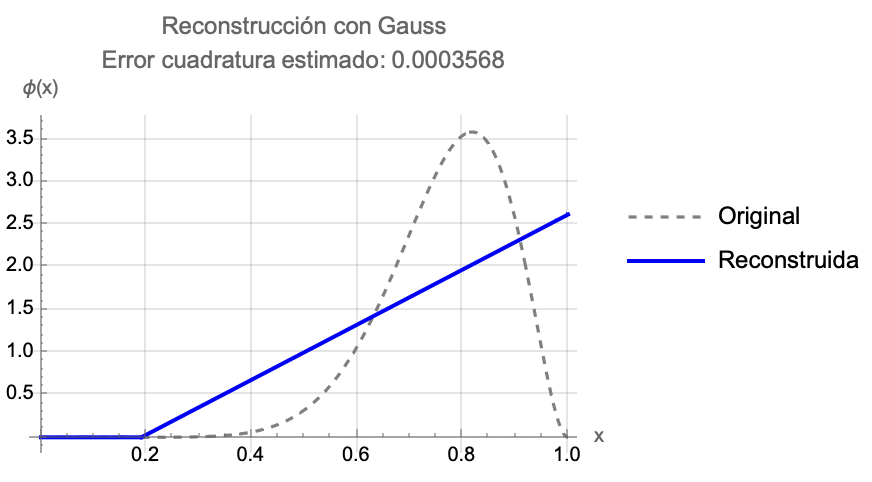
\includegraphics[height = 4.5 cm]{Gauss/Mu2P10.png}
        \caption{Aproximación para 2 momentos}
        \label{Gauss/Mu2P10}
    \end{minipage}
    \hfill
    \begin{minipage}{0.45\textwidth}
        \centering
        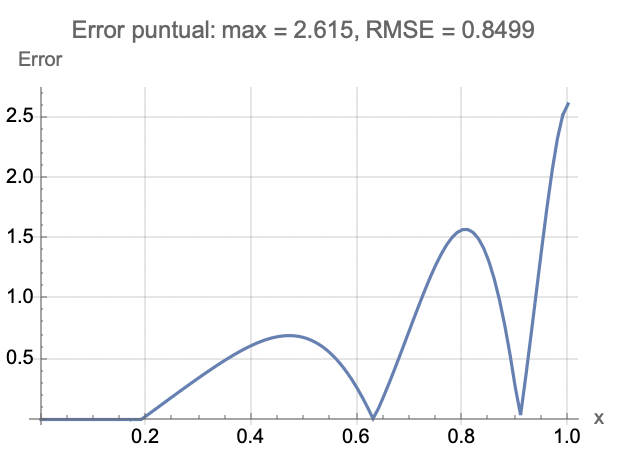
\includegraphics[height = 4.5 cm]{Gauss/ErrMu2P10.png}
        \caption{Error puntual en la aproximación. Diferencia entre $\phi(x)$ y $f(x)$.}
        \label{Gauss/ErrMu2P10}
    \end{minipage}
\end{figure}
\begin{figure}[H]
 \centering
 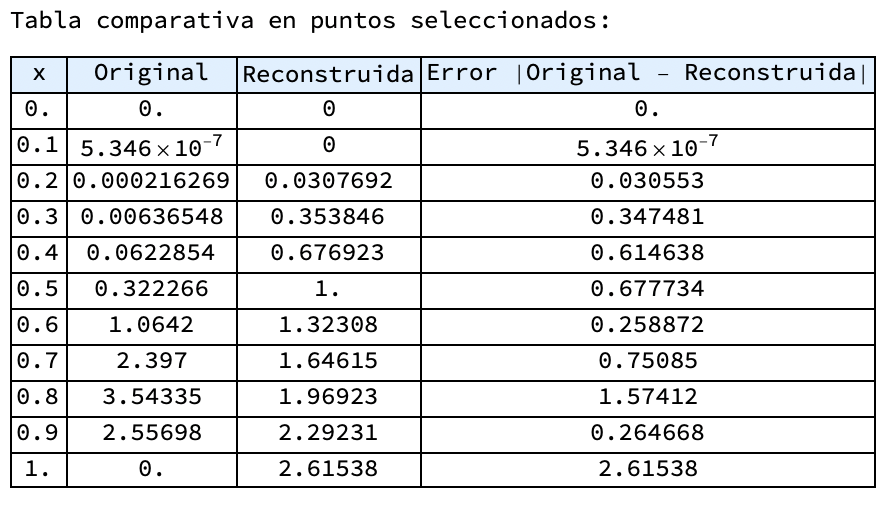
\includegraphics[height = 5.0 cm]{Gauss/TComMu2P10.png}
 \caption{Tabla comparativa entre función original y reconstruida para 2 momentos.}
 \label{Gauss/TComMu2P10}
 \end{figure}
\begin{figure}[H]
    \centering
    \begin{minipage}
    {0.45\textwidth}
        \centering
        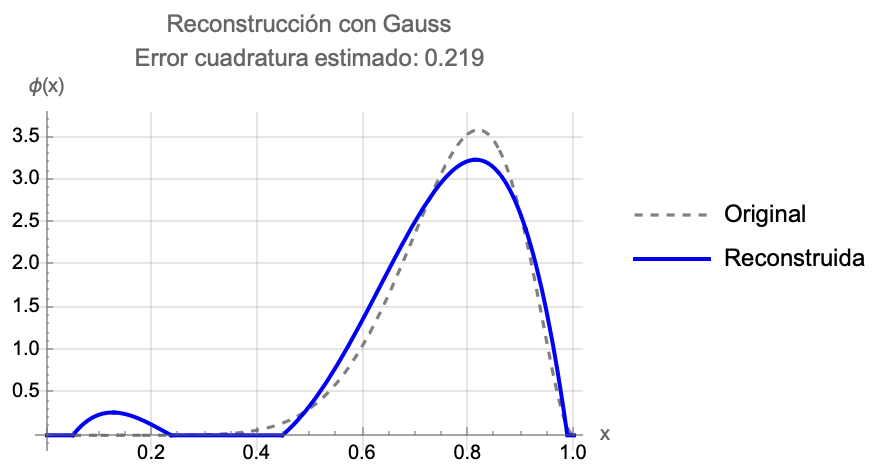
\includegraphics[height = 4.5 cm]{Gauss/Mu5P10.png}
        \caption{Aproximación para 5 momentos}
        \label{Gauss/Mu5P10}
    \end{minipage}
    \hfill
    \begin{minipage}{0.45\textwidth}
        \centering
        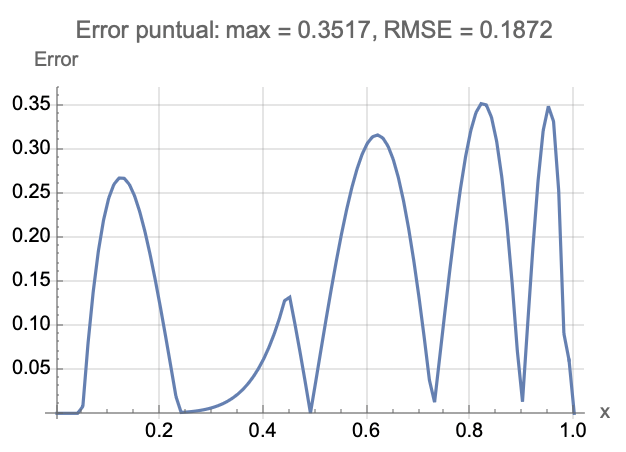
\includegraphics[height = 4.5 cm]{Gauss/ErrMu5P10.png}
        \caption{Error puntual en la aproximación. Diferencia entre $\phi(x)$ y $f(x)$.}
        \label{Gauss/ErrMu5P10}
    \end{minipage}
\end{figure}
\begin{figure}[H]
 \centering
 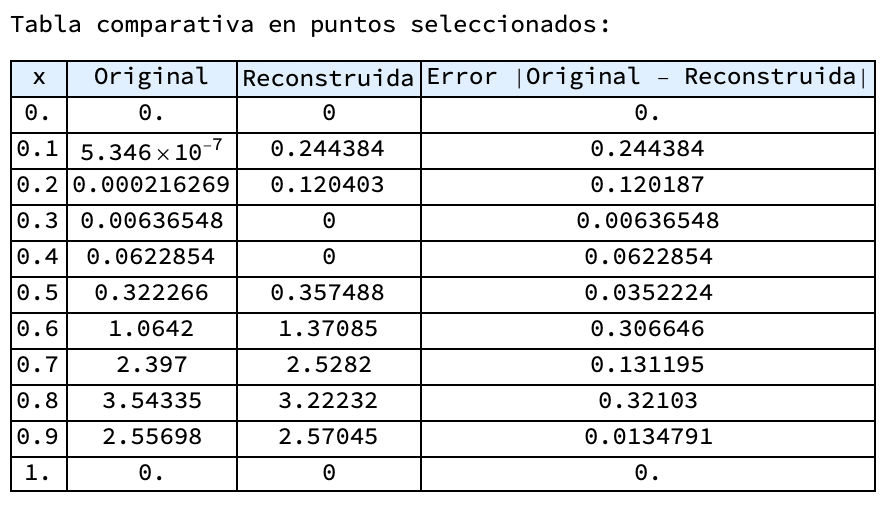
\includegraphics[height = 5.0 cm]{Gauss/TComMu5P10.png}
 \caption{Tabla comparativa entre función original y reconstruida para 5 momentos.}
 \label{Gauss/TComMu5P10}
 \end{figure}
\begin{figure}[H]
    \centering
    \begin{minipage}
    {0.45\textwidth}
        \centering
        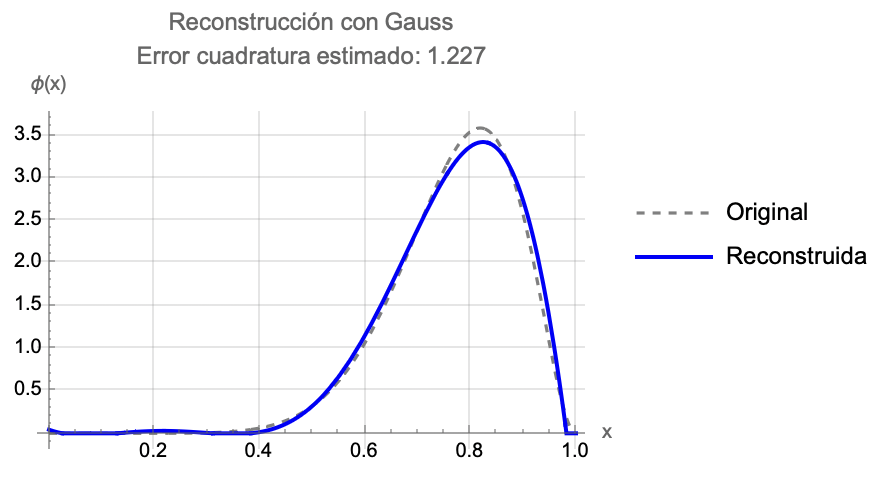
\includegraphics[height = 4.5 cm]{Gauss/Mu10P10.png}
        \caption{Aproximación para 10 momentos}
        \label{Gauss/Mu10P10}
    \end{minipage}
    \hfill
    \begin{minipage}{0.45\textwidth}
        \centering
        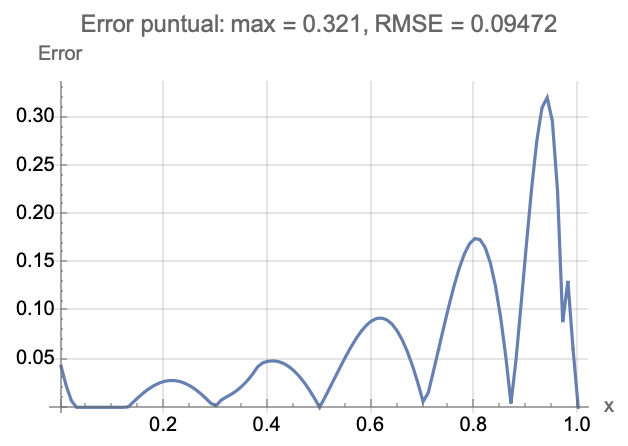
\includegraphics[height = 4.5 cm]{Gauss/ErrMu10P10.png}
        \caption{Error puntual en la aproximación. Diferencia entre $\phi(x)$ y $f(x)$.}
        \label{Gauss/ErrMu10P10}
    \end{minipage}
\end{figure}
\begin{figure}[H]
 \centering
 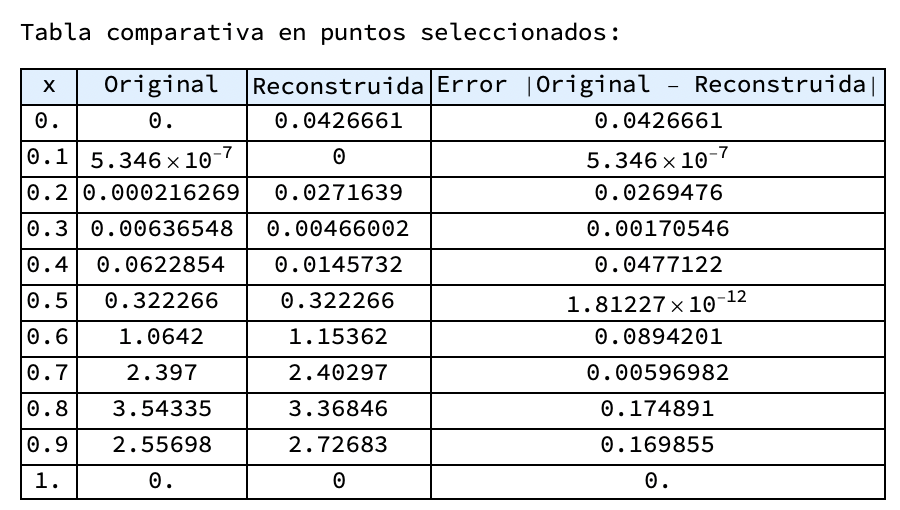
\includegraphics[height = 5.0 cm]{Gauss/TComMu10P10.png}
 \caption{Tabla comparativa entre función original y reconstruida para 10 momentos.}
 \label{Gauss/TComMu10P10}
 \end{figure}


Obteniendo una cota superior del error de integración de $0.0003568$ para $2$ momentos, $0.219$ para $5$ momentos y $1.227$ para $10$ momentos.

Se obtuvo la siguiente tabla de errores para $1$ a $10$ momentos.
\begin{figure}[H]
 \centering
 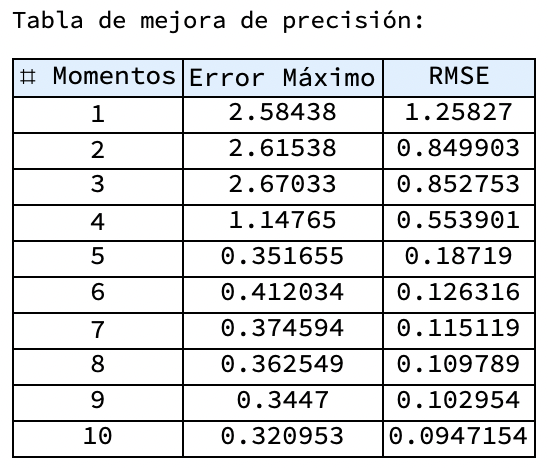
\includegraphics[height = 4.0 cm]{Gauss/TErrP10.png}
 \caption{Tabla comparativa entre función original y reconstruida para 10 puntos.}
 \label{Gauss/TErrP10}
 \end{figure}

Esto es:
\begin{figure}[H]
 \centering
 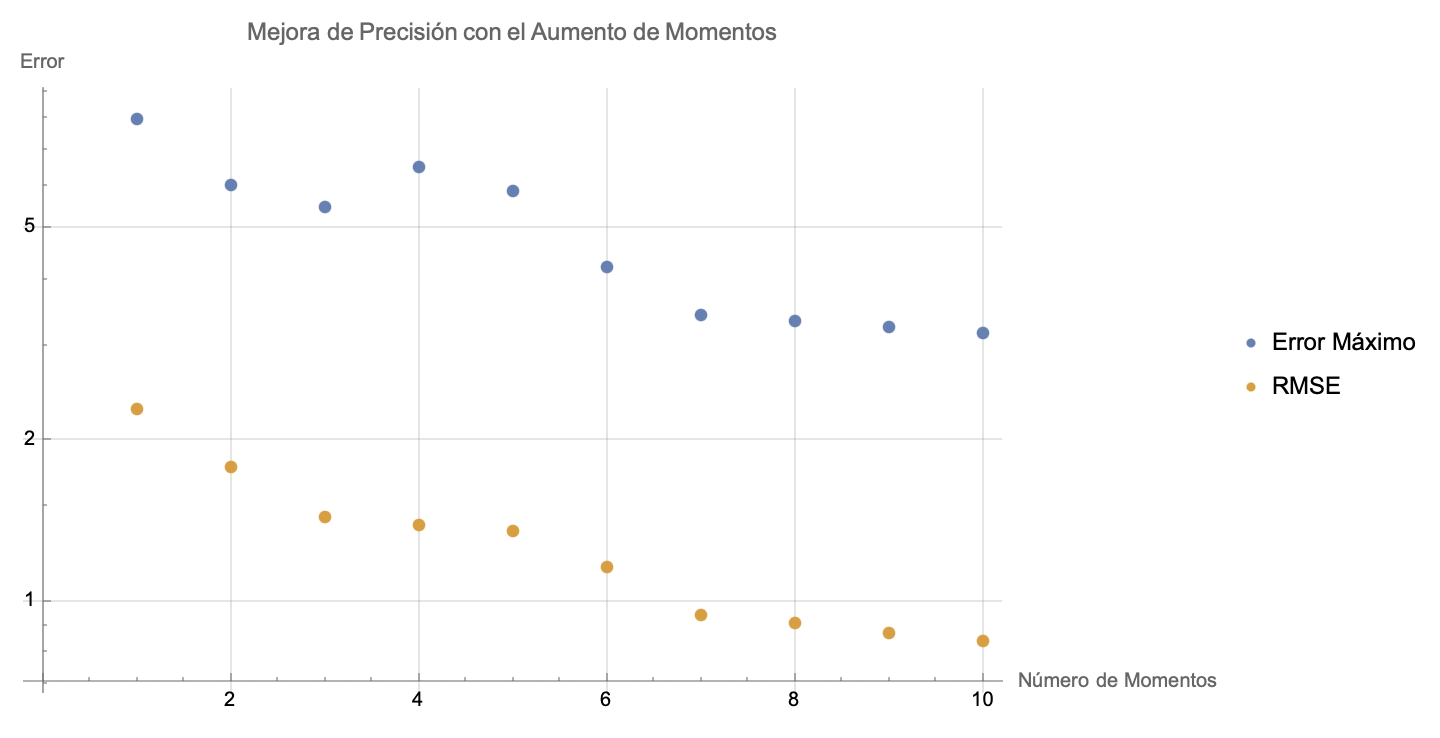
\includegraphics[height = 7.0 cm]{Gauss/PreP30.png}
 \caption{Errores vs. Número de momentos para 10 puntos.}
 \label{Gauss/PreP30}
 \end{figure}

Para $30$ puntos se consideraron los casos en los que se tienen $2$, $5$ y $10$ momentos conocidos de la función.

\begin{figure}[H]
    \centering
    \begin{minipage}
    {0.45\textwidth}
        \centering
        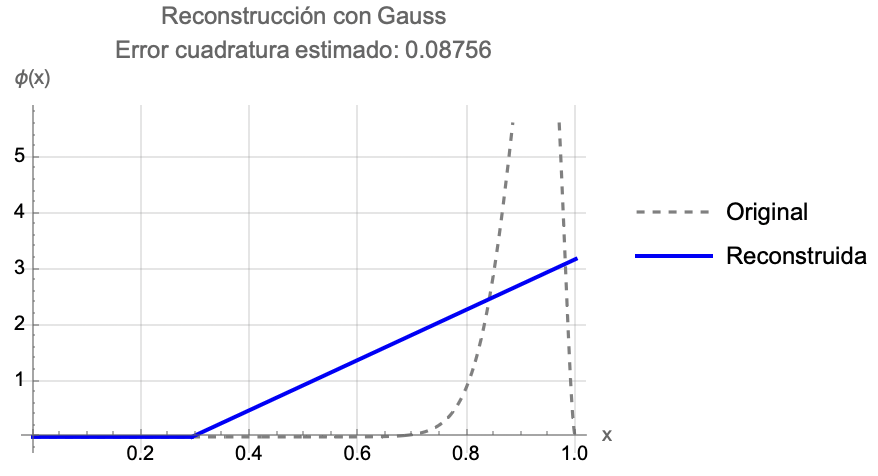
\includegraphics[height = 4.5 cm]{Gauss/Mu2P30.png}
        \caption{Aproximación para 2 momentos}
        \label{Gauss/Mu2P30}
    \end{minipage}
    \hfill
    \begin{minipage}{0.45\textwidth}
        \centering
        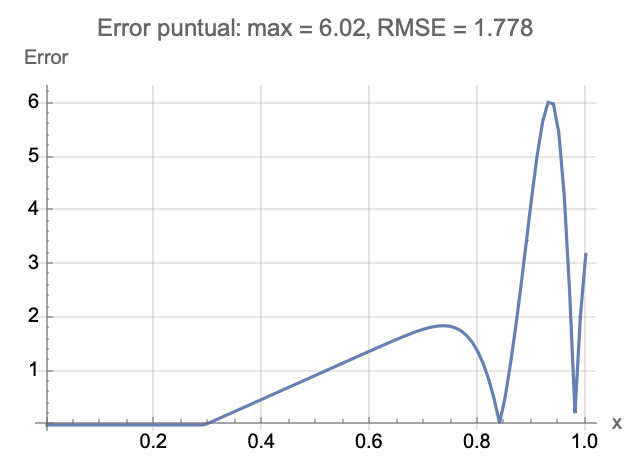
\includegraphics[height = 4.5 cm]{Gauss/ErrMu2P30.png}
        \caption{Error puntual en la aproximación. Diferencia entre $\phi(x)$ y $f(x)$.}
        \label{Gauss/ErrMu2P30}
    \end{minipage}
\end{figure}
\begin{figure}[H]
 \centering
 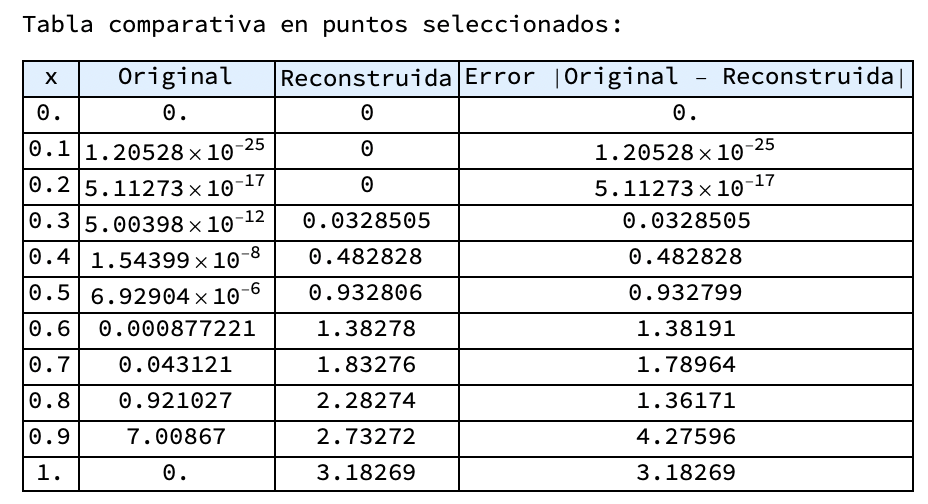
\includegraphics[height = 5.0 cm]{Gauss/TComMu2P30.png}
 \caption{Tabla comparativa entre función original y reconstruida para 2 momentos.}
 \label{Gauss/TComMu2P30}
 \end{figure}
\begin{figure}[H]
    \centering
    \begin{minipage}
    {0.45\textwidth}
        \centering
        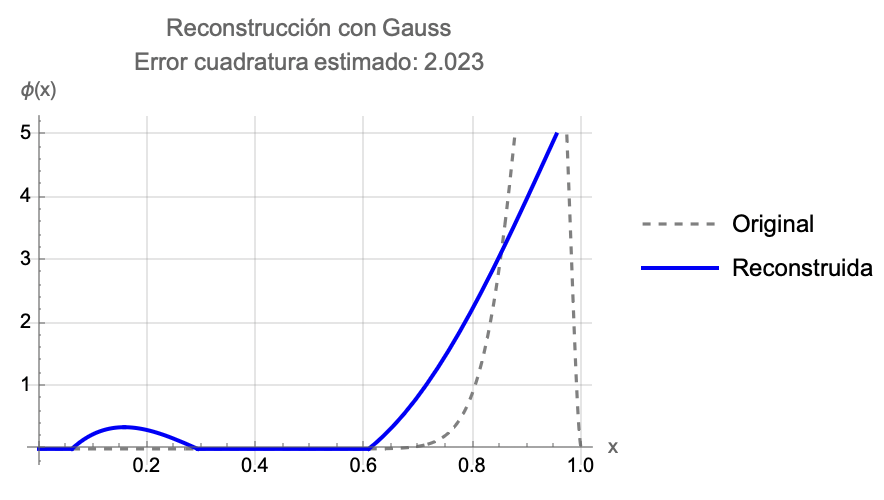
\includegraphics[height = 4.5 cm]{Gauss/Mu5P30.png}
        \caption{Aproximación para 5 momentos}
        \label{Gauss/Mu5P30}
    \end{minipage}
    \hfill
    \begin{minipage}{0.45\textwidth}
        \centering
        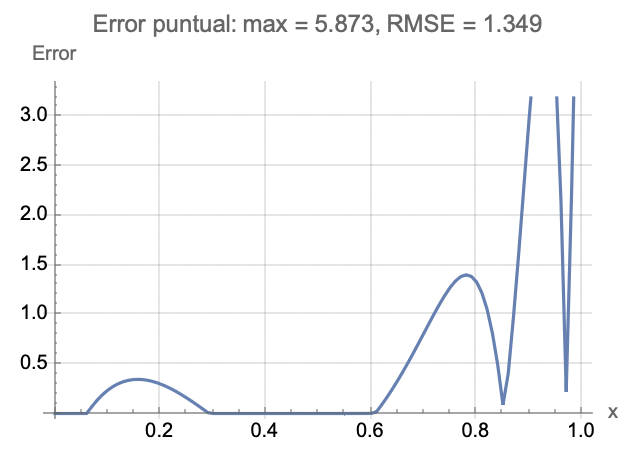
\includegraphics[height = 4.5 cm]{Gauss/ErrMu5P30.png}
        \caption{Error puntual en la aproximación. Diferencia entre $\phi(x)$ y $f(x)$.}
        \label{Gauss/ErrMu5P30}
    \end{minipage}
\end{figure}
\begin{figure}[H]
 \centering
 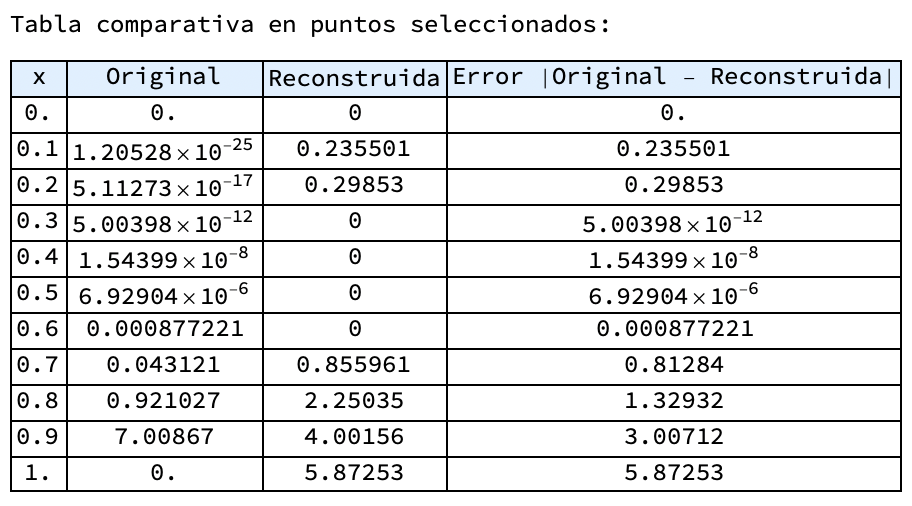
\includegraphics[height = 5.0 cm]{Gauss/TComMu5P30.png}
 \caption{Tabla comparativa entre función original y reconstruida para 5 momentos.}
 \label{Gauss/TComMu5P30}
 \end{figure}
\begin{figure}[H]
    \centering
    \begin{minipage}
    {0.45\textwidth}
        \centering
        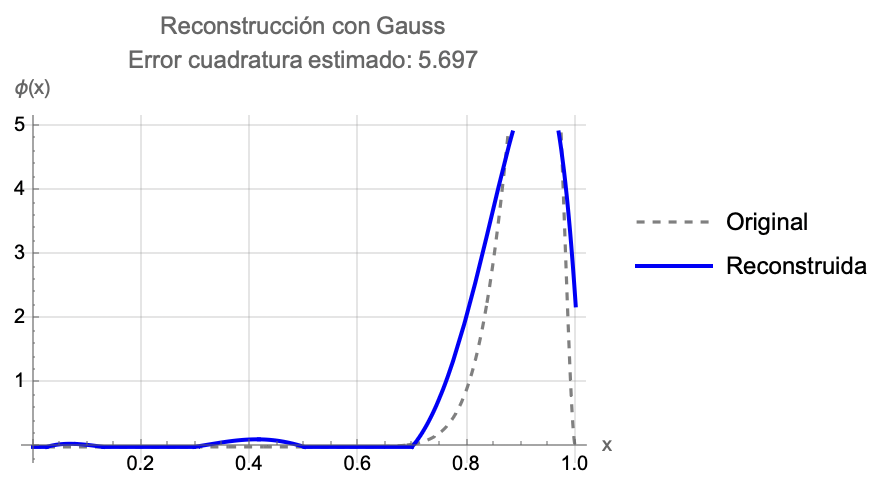
\includegraphics[height = 4.5 cm]{Gauss/Mu10P30.png}
        \caption{Aproximación para 10 momentos}
        \label{Gauss/Mu10P30}
    \end{minipage}
    \hfill
    \begin{minipage}{0.45\textwidth}
        \centering
        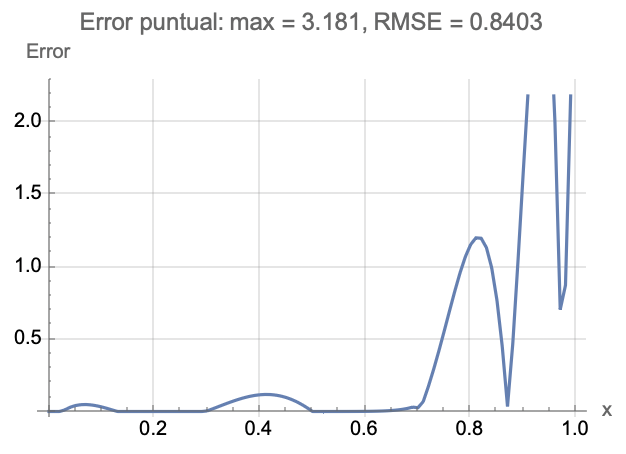
\includegraphics[height = 4.5 cm]{Gauss/ErrMu10P30.png}
        \caption{Error puntual en la aproximación. Diferencia entre $\phi(x)$ y $f(x)$.}
        \label{Gauss/ErrMu10P30}
    \end{minipage}
\end{figure}
\begin{figure}[H]
 \centering
 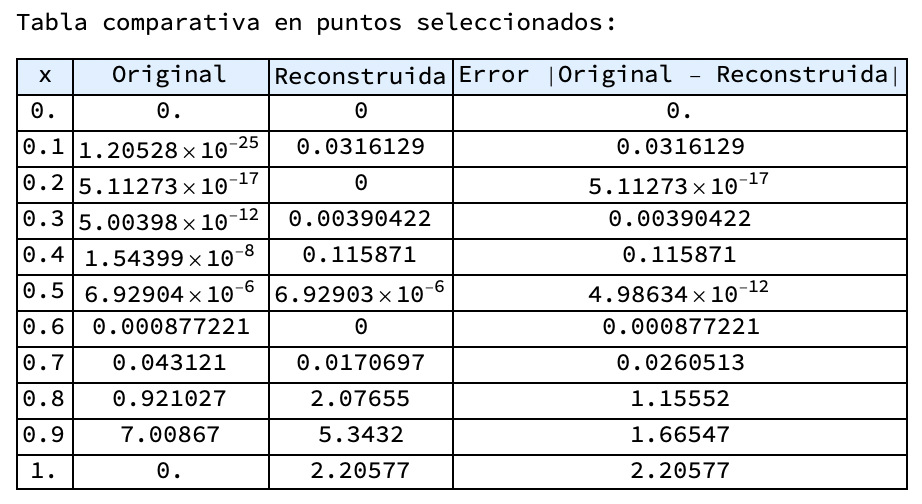
\includegraphics[height = 5.0 cm]{Gauss/TComMu10P30.png}
 \caption{Tabla comparativa entre función original y reconstruida para 10 momentos.}
 \label{Gauss/TComMu10P30}
 \end{figure}


Obteniendo una cota superior del error de integración de $0.08758$ para $2$ momentos, $2.023$ para $5$ momentos y $5.697$ para $10$ momentos.

Se obtuvo la siguiente tabla de errores para $1$ a $10$ momentos.
\begin{figure}[H]
 \centering
 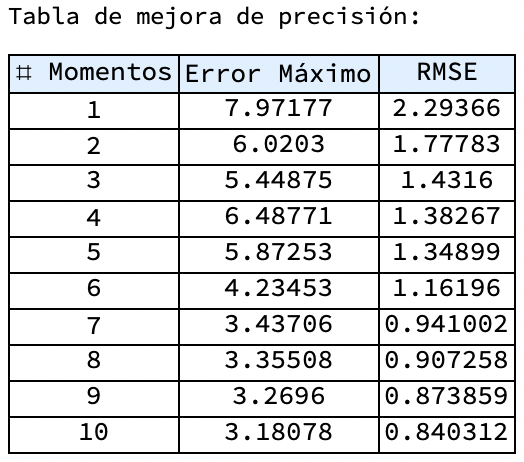
\includegraphics[height = 4.0 cm]{Gauss/TErrP30.png}
 \caption{Tabla comparativa entre función original y reconstruida para 2 momentos 30 puntos.}
 \label{Gauss/TErrP30}
 \end{figure}

Esto es:
\begin{figure}[H]
 \centering
 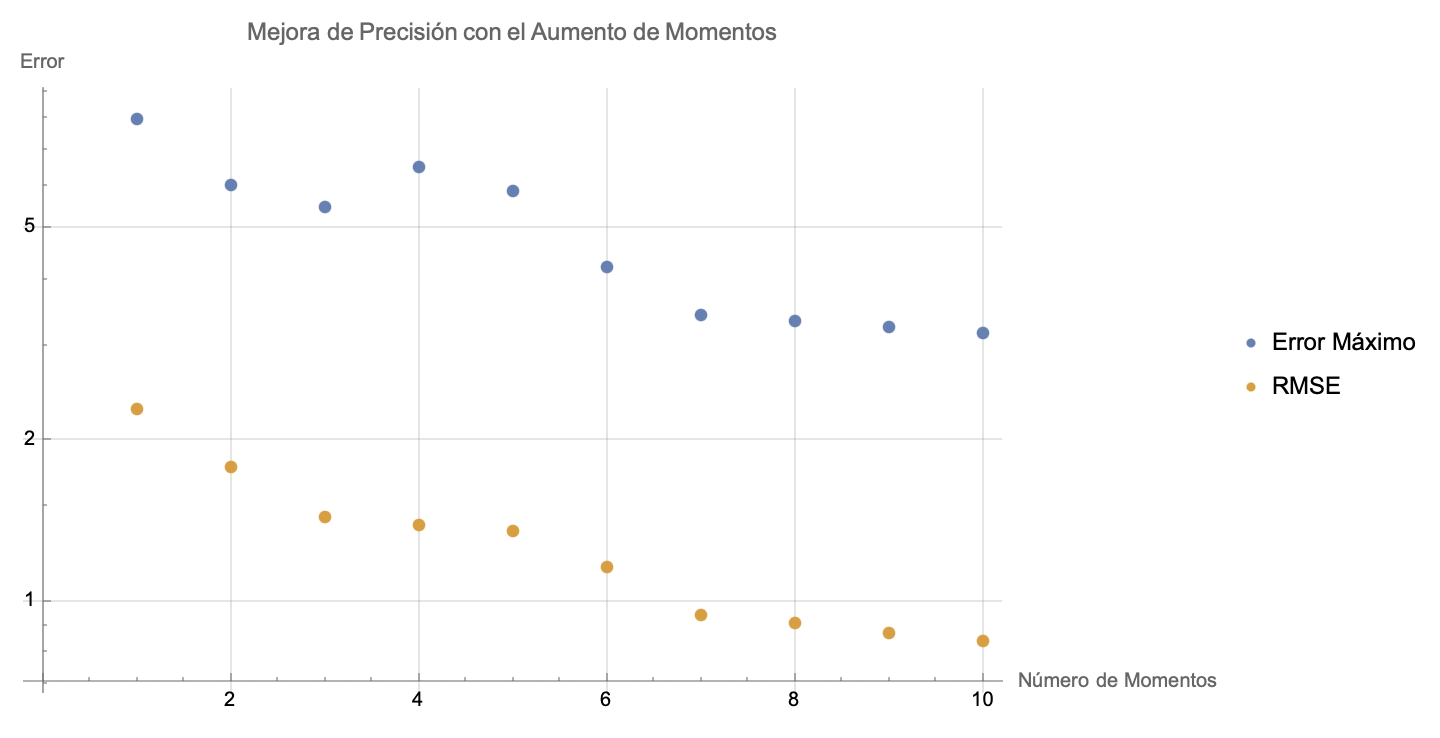
\includegraphics[height = 7.0 cm]{Gauss/PreP30.png}
 \caption{Errores vs. Número de momentos para 30 puntos.}
 \label{Gauss/PreP30}
 \end{figure}

Para $75$ puntos se consideraron los casos en los que se tienen $2$, $5$ y $10$ momentos conocidos de la función.

\begin{figure}[H]
    \centering
    \begin{minipage}
    {0.45\textwidth}
        \centering
        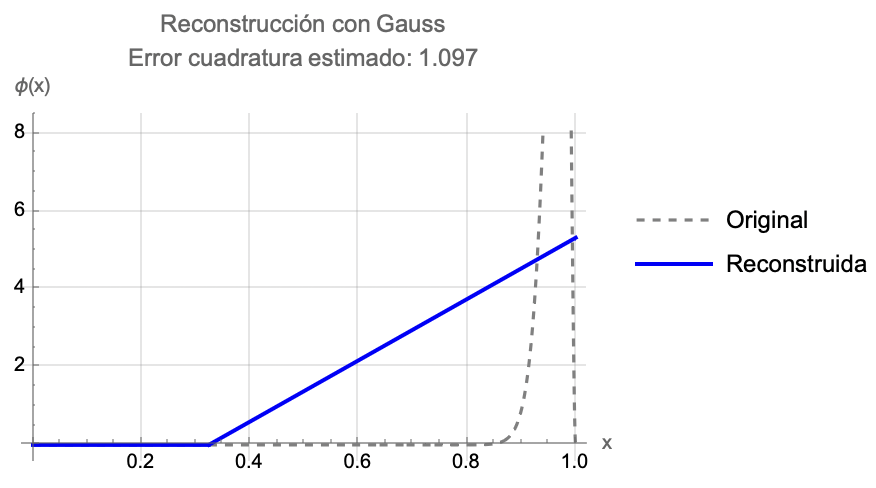
\includegraphics[height = 4.5 cm]{Gauss/Mu2P75.png}
        \caption{Aproximación para 2 momentos}
        \label{Gauss/Mu2P75}
    \end{minipage}
    \hfill
    \begin{minipage}{0.45\textwidth}
        \centering
        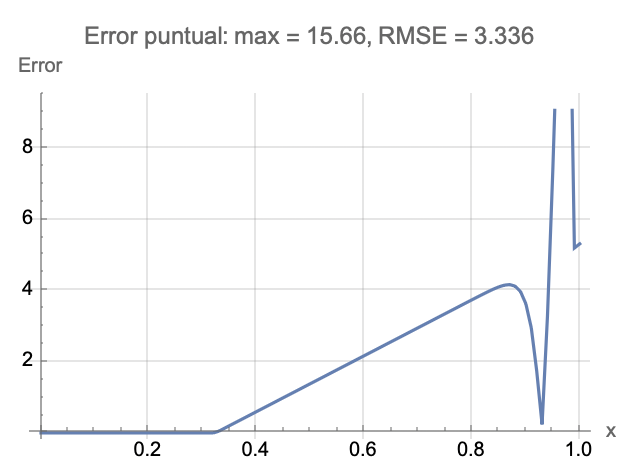
\includegraphics[height = 4.5 cm]{Gauss/ErrMu2P75.png}
        \caption{Error puntual en la aproximación. Diferencia entre $\phi(x)$ y $f(x)$.}
        \label{Gauss/ErrMu2P75}
    \end{minipage}
\end{figure}
\begin{figure}[H]
 \centering
 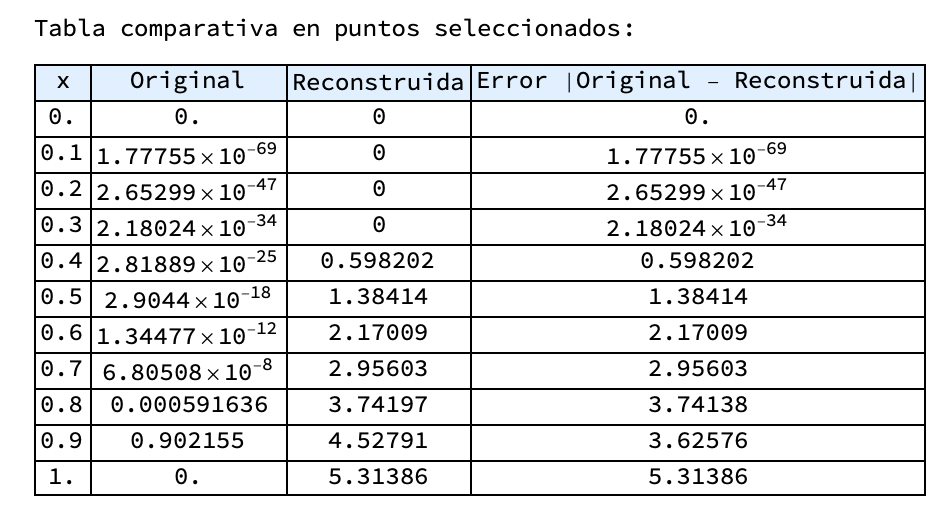
\includegraphics[height = 5.0 cm]{Gauss/TComMu2P75.png}
 \caption{Tabla comparativa entre función original y reconstruida para 2 momentos.}
 \label{Gauss/TComMu2P75}
 \end{figure}
\begin{figure}[H]
    \centering
    \begin{minipage}
    {0.45\textwidth}
        \centering
        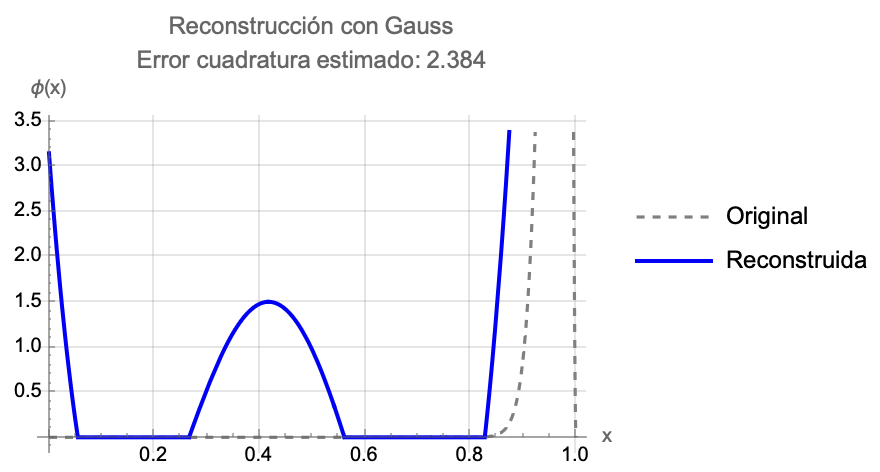
\includegraphics[height = 4.5 cm]{Gauss/Mu5P75.png}
        \caption{Aproximación para 5 momentos}
        \label{Gauss/Mu5P75}
    \end{minipage}
    \hfill
    \begin{minipage}{0.45\textwidth}
        \centering
        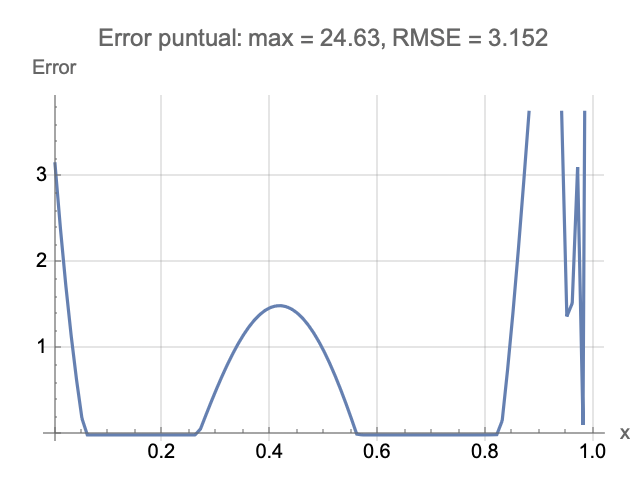
\includegraphics[height = 4.5 cm]{Gauss/ErrMu5P75.png}
        \caption{Error puntual en la aproximación. Diferencia entre $\phi(x)$ y $f(x)$.}
        \label{Gauss/ErrMu5P75}
    \end{minipage}
\end{figure}
\begin{figure}[H]
 \centering
 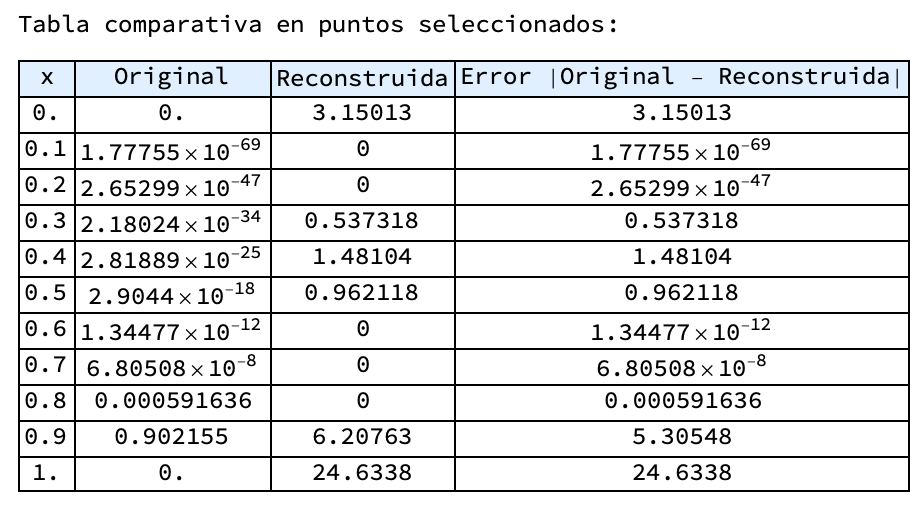
\includegraphics[height = 5.0 cm]{Gauss/TComMu5P75.png}
 \caption{Tabla comparativa entre función original y reconstruida para 5 momentos.}
 \label{Gauss/TComMu5P75}
 \end{figure}
\begin{figure}[H]
    \centering
    \begin{minipage}
    {0.45\textwidth}
        \centering
        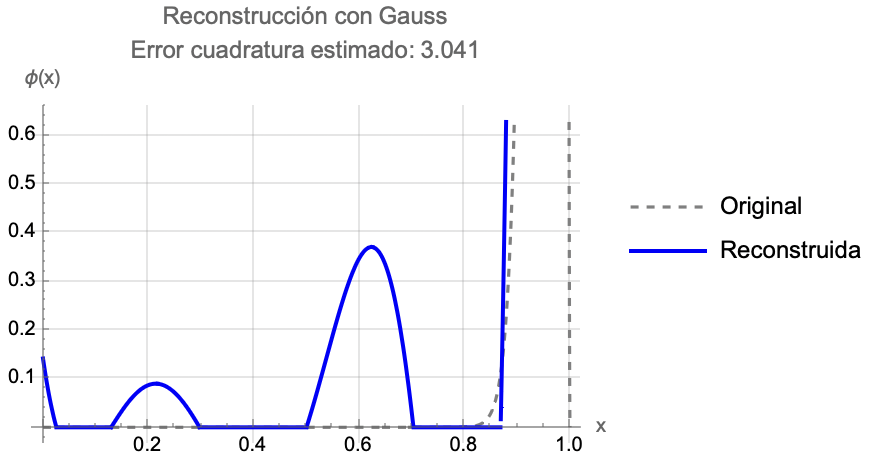
\includegraphics[height = 4.5 cm]{Gauss/Mu10P75.png}
        \caption{Aproximación para 10 momentos}
        \label{Gauss/Mu10P75}
    \end{minipage}
    \hfill
    \begin{minipage}{0.45\textwidth}
        \centering
        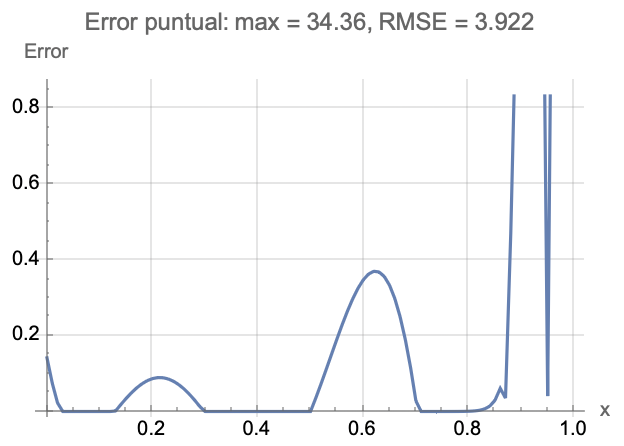
\includegraphics[height = 4.5 cm]{Gauss/ErrMu10P75.png}
        \caption{Error puntual en la aproximación. Diferencia entre $\phi(x)$ y $f(x)$.}
        \label{Gauss/ErrMu10P75}
    \end{minipage}
\end{figure}
\begin{figure}[H]
 \centering
 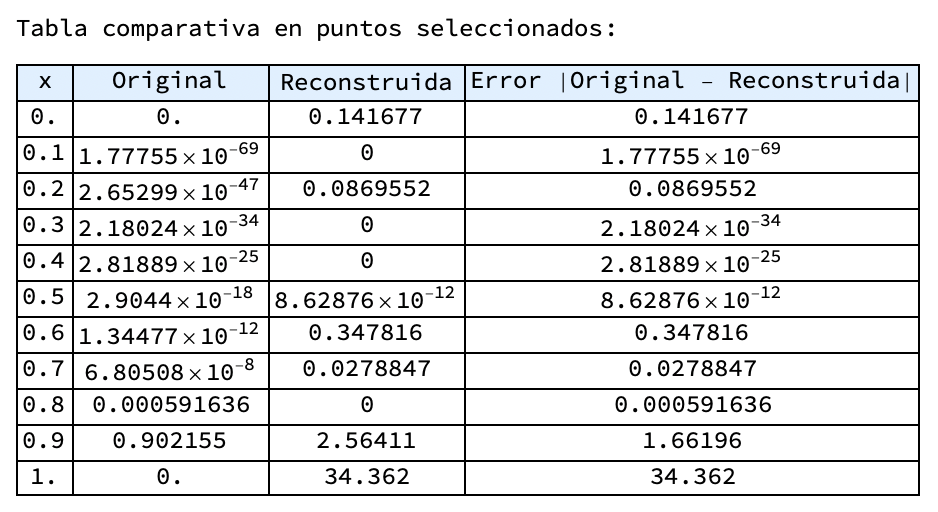
\includegraphics[height = 5.0 cm]{Gauss/TComMu10P75.png}
 \caption{Tabla comparativa entre función original y reconstruida para 10 momentos.}
 \label{Gauss/TComMu10P75}
 \end{figure}


Obteniendo una cota superior del error de integración de $1.097$ para $2$ momentos, $2.384$ para $5$ momentos y $3.041$ para $10$ momentos.

Se obtuvo la siguiente tabla de errores para $1$ a $10$ momentos.
\begin{figure}[H]
 \centering
 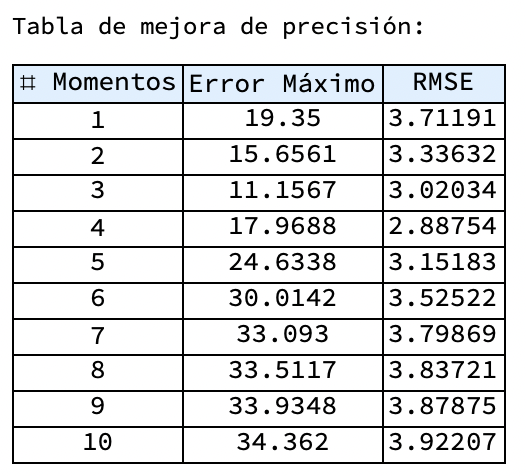
\includegraphics[height = 4.0 cm]{Gauss/TErrP75.png}
 \caption{Tabla comparativa entre función original y reconstruida para 75 puntos.}
 \label{Gauss/TErrP75}
 \end{figure}

Esto es:
\begin{figure}[H]
 \centering
 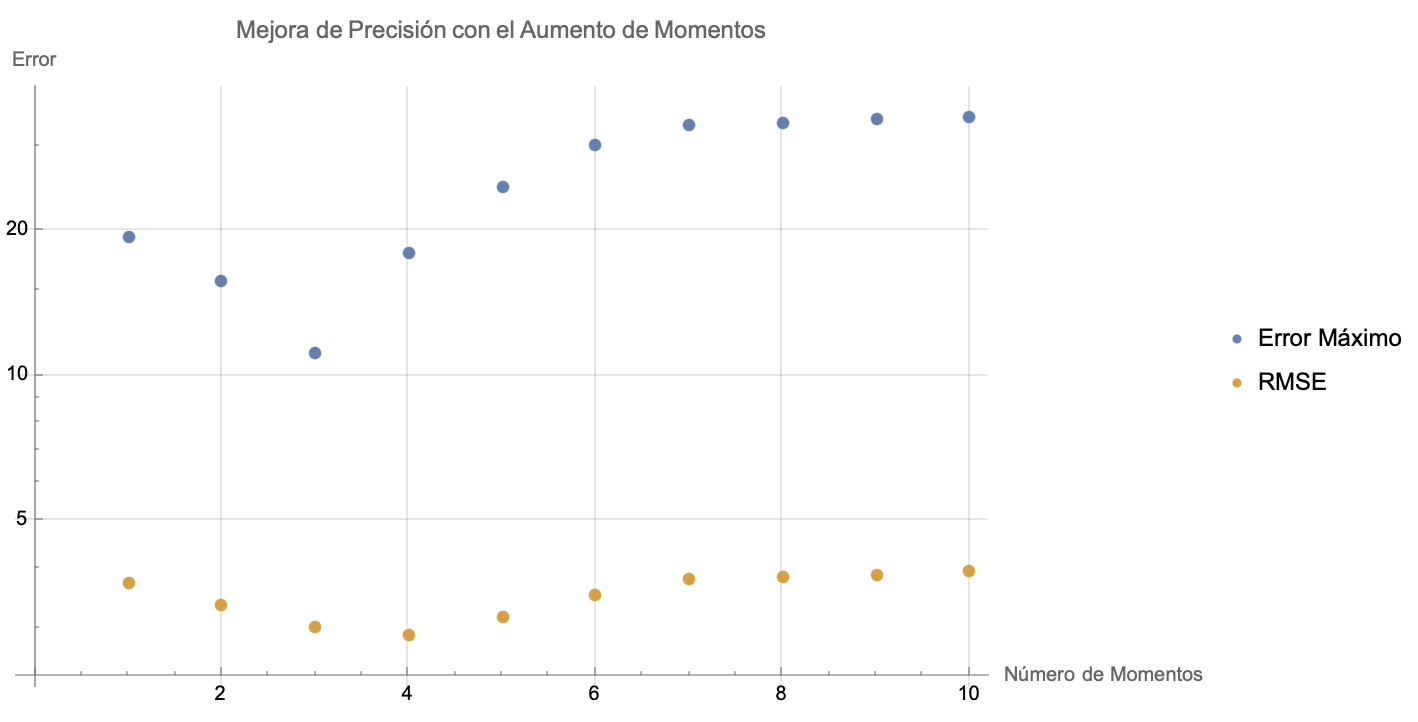
\includegraphics[height = 7.0 cm]{Gauss/PreP75.png}
 \caption{Errores vs. Número de momentos para 75 puntos.}
 \label{Gauss/PreP75}
 \end{figure}


Es posible comparar la eficiencia de los tres métodos utilizados mediante el valor de RMSE de sus aproximaciones para un número de puntos dado, a medida que aumenta el número de momentos conocidos. Se obtiene lo siguiente:
\begin{figure}[H]
    \centering
    \begin{minipage}
    {0.45\textwidth}
        \centering
        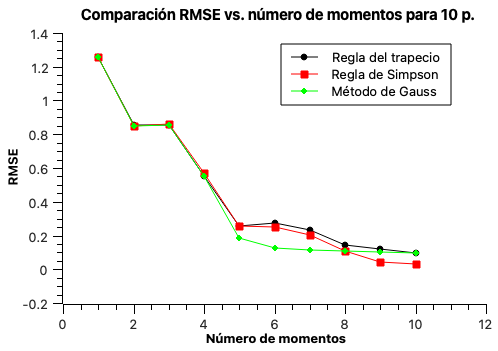
\includegraphics[height = 3.5 cm]{RMSE/RMSE10P.png}
        \caption{Comparación de RMSE para 10 puntos y 10 primeros momentos.}
        \label{RMSE/RMSE10P}
    \end{minipage}
    \hfill
    \begin{minipage}{0.45\textwidth}
        \centering
        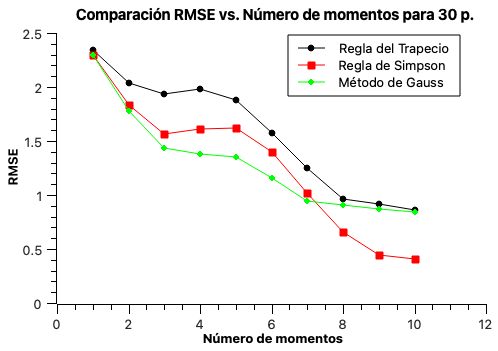
\includegraphics[height = 3.5 cm]{RMSE/RMSE30P.png}
        \caption{Comparación de RMSE para 30 puntos y 10 primeros momentos.}
        \label{RMSE/RMSE30P}
    \end{minipage}
\end{figure}
\begin{figure}[h]
 \centering
 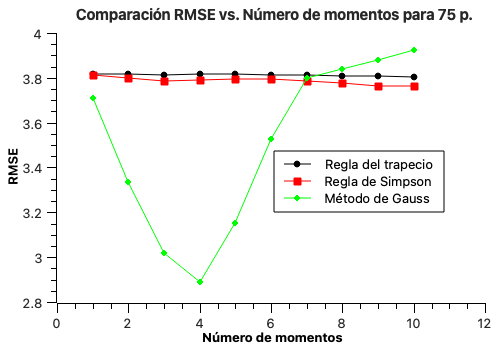
\includegraphics[height = 3.5 cm]{RMSE/RMSE75P.png}
 \caption{Comparación de RMSE para 75 puntos y 10 primeros momentos.}
 \label{RMSE/RMSE75P}
 \end{figure}

Para un número bajo de puntos, los tres métodos se comportan de forma muy similar y ninguno es claramente más eficiente que los demás. El RMSE de la regla del trapecio y la regla de Simpson tienen un comportamiento similar. Sin embargo, la regla de Simpson brinda en cada caso un RMSE más bajo que la regla del trapecio a medida que aumenta el número de momentos conocidos.

A medida que se estudian valores más altos de $N_p$ se observa la clara ventaja que ofrece la regla de Simpson sobre la regla del trapecio, y se observa una clara diferencia entre estos dos métodos (que siguen un comportamiento similar) y el método de Gauss, cuyo RMSE disminuye hasta un número ideal de momentos, cuando el RMSE es mínimo. Luego de este valor ideal de momentos conocidos el RMSE aumenta nuevamente, lo que sugiere que el método de Gauss utilizado para valores grandes de $N_p$ necesita de pocos momentos conocidos para ser preciso, y de hecho, se comporta más eficiente para pocos momentos conocidos que para un número alto de ellos. Para los otros métodos este comportamiento también ocurre, sin embargo el número ideal de momentos conocidos es mucho más alto para un número de puntos bajo. Esto es, se requiere de dimensiones de $\vec{\mu}_n$ más pequeñas para obtener resultados similares con el método de Gauss a comparación de los otros métodos, es decir, para un número de puntos dado brinda en general, aproximaciones igual de precisas para un número de momentos más bajo.

En cuanto a la precisión de las reconstrucciones en los distintos puntos de la función $\phi(x)$ se obtiene una discrepancia mayor para esta distribución en el extremo derecho en la mayoría de los casos. Lo que se corresponde con el fenómeno de Runge, cuando los polinomios tienden a volverse inestables en los extremos del intervalo.  

En cuanto al error global de cuadratura en los métodos utilizados, se obtiene que este es mayor a medida que aumenta el número de momentos conocidos para un número de puntos dado. Esto es completamente válido y se corresponde con el análisis matemático del capítulo \ref{sec:metodologia}, pues añadir momentos implica integrar $x^n\phi(x)$ de mayor grado de complejidad numérica.

Este aumento del error global con el número de momentos se observa incluso para el método de Gauss, en donde no se calcula el error con la fórmula de la derivada $2n$-ésima sino mediante la comparación de las reconstrucciones de $n$ y $n-1$, estimando un error empírico que se corresponde proporcionalmente con el error teórico.


\chapter{Conclusiones y futuros trabajos}
\label{sec:conclusiones}

La reconstrucción precisa de las PDFs es esencial para mejorar la exactitud de las predicciones teóricas y obtener una mejor comprensión de la física a nivel subatómico. La PDF de una partícula $i$, $f_i$ puede entenderse como el peso de los coeficientes de las funciones de estructura electromagnética para esa partícula, siendo las funciones de estructura electromagnética del hadrón, una suma de todas estas contribuciones ponderadas de acuerdo al $f_i$ de cada partícula constituyente. Puesto que las funciones de estructura electromagnética forman parte del tensor hadrónico, conocerlas es crucial para paramatrizarlo y por tanto, para calcular la sección eficaz como el producto del tensor hadrónico y leptónico para la interacción. 

Estudiar los distintos métodos de integración numérica para la reconstrucción de PDFs, resultó ser una opción factible, pues tiene un bajo coste computacional, basándose principalmente en calcular el peso de los coeficientes asociados a la aproximación del cálculo de la integral de la función, para el método elegido.

 El método más eficiente para aproximar mediante polinomios una función de distribución de partones resultó ser el método de Gauss, pues para un número dado de puntos, necesita de menos momentos conocidos para dar un resultado comparable al de los otros dos para mayor número de momentos. Tanto la regla del trapecio como la regla de Simpson comparten una eficacia similar, sin embargo, bajo las mismas condiciones se observa un RMSE ligeramente más pequeño para la regla de Simpson en cualquiera de los casos.

Si para un número de puntos dado se supera en cualesquiera de los tres métodos un cierto número de momentos conocido en la aproximación, esta tenderá a aumentar su RMSE, es decir tenderá a ser una peor estimación de la curva original.


% esta versión usa Bibtex para generar las referencias que están en archivo
% adjunto con el nombre referencias.bib.  Hay varios estilos, los básicos son:
% abbrv, acm, alpha, apalike, ieeetr, plain, siam, unsrt
\nocite{*}
\bibliographystyle{ieeetr}% otras opciones {plain}
\bibliography{ref}
\end{document}


%%% Local Variables:
%%% mode: latex
%%% TeX-master: t
%%% End:
